\documentclass[letterpaper]{book}
\usepackage{graphicx}
\usepackage{amsmath}
\usepackage{wrapfig}
\usepackage{floatflt}
\usepackage{listings}
\usepackage{xcolor}
\usepackage{nameref}
\usepackage{textcomp}
\usepackage{tabularx} 
\usepackage{url}


\begin{document}

\title{ BK Radar Sampler Simulator (BKRadSim) }
\maketitle

\section{Summary}




BKRadSim is a signal level simulation software library specifically designed for naval radars. Its end product is the raw signal sampling after reception and analog to digital conversion, which can then be used as input to a digital processing algorithm designed by the user. The main motivation behind the library is to create a tool for learning or developing tracking algorithms. It is mainly written for C++14 by with bindings to Python as well. The simulator may be called sequentially, but also parallell to any digital processing in order to test real time track performance. 

With recent developments in statistics, for which I mention artifical intelligence (AI), new avenues with regards to detection and classification have openeded up. The main limitation in using AI, is that is requires a substantial amount of data. Aquiring experimental data of this magnitude may prove both costly, either through field testing or the purchase of proprietary software and hardware equipment. By making an open source simulator available for this purpose, being able to create the very data artifically, initial studying and development of track algorithms can be done by anyone. 





\tableofcontents

\chapter{Introduction}
\section{Motivation and Functionality}
This library supports signal level simulation of surface based radars with rotating antenna. The functionality of these radars is to provide 2D surveillance of its surroundings with regards to maritime and airborne traffic. 

A radar works by emitting and receiving radiosignals for the purpose of area surveillance. The targets are usually coastlines, marine vessels or aircraft. Unfortunately, almost anything will echo back. As well as boats and airplanes this includes land, rock, cars, any installations, trees, buildings, the sea, rain drops, birds and even insects. A detection system will need to distinguish between interesting and non-interesting backscatterers. In these days, the hardware of most radars can deliver raw received signal measurements digitally. These signals, although electronically processed by amplifications and filtering, are still very raw data and need \textit{digital processing} in order to create meaningful output. That processing may produce per-scan detections, referred to as \textit{contacts} or \textit{plots}, but also more complicated classifications known as \textit{tracks}, containing dynamic data as well.

\begin{figure}
  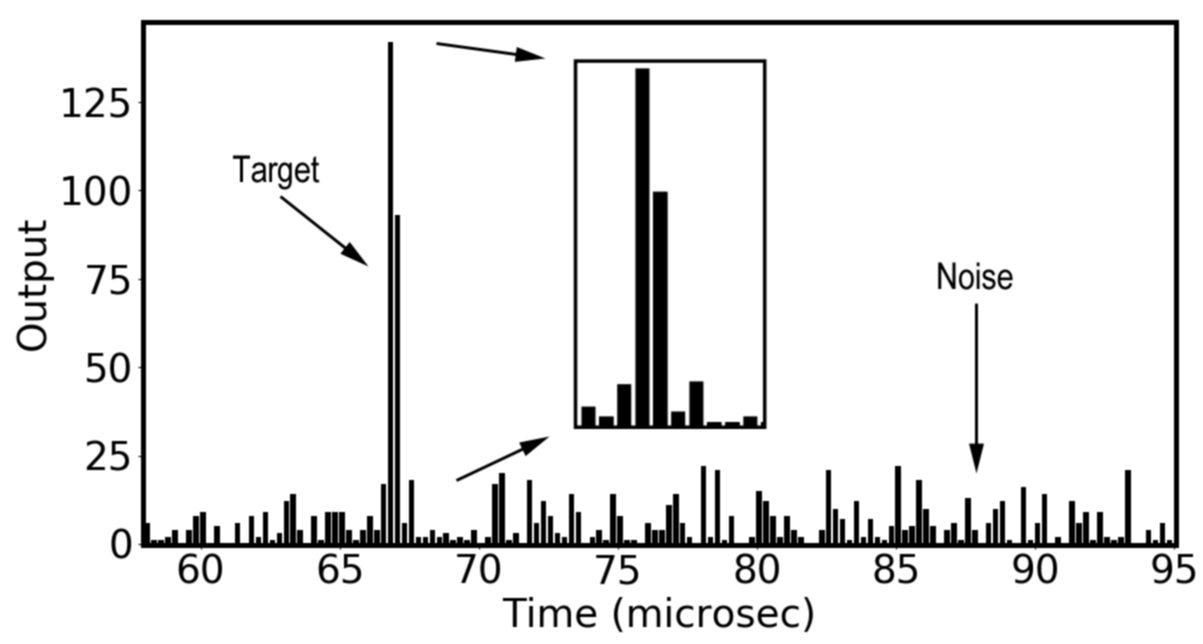
\includegraphics[width=8cm]{noise_target_3_c.png}
  \caption{\textit{10-bit signal measurements as function of time during reception of a single pulse.}}
  \label{fig:noise_target}
\end{figure}

Studying digital processing or developing for technological use requires data to train on. What is needed is something that returns radar signals in the form of contacts, or even raw or digitally sampled signals for the tracking developer to work on. This datastream would ideally be in real time so as to assert that the signal processing procedure can keep pace with the continuous signal reception. BKRadSim attempts to do this by simulating the raw sampled signal from the received pulsed signal, with a system for connecting to a program for signal processing. Figure \ref{fig:noise_target} provides a glimpse of what kind of data is produced: raw signal samplings recorded after a single pulse emission. Most of the data is noise, but there is also a powerful signal originating from a target. The simulator can provide near-realtime deliverance during the continuous rotation of the radar antenna: one array of signal samplings after each emitted pulse. The user -- a signal process programmer -- can then use it to simulate the total radar performance, from pulse emission to track generation and handling. 

This is not a computer program, but a core library intended for radar tracking development.


\section{Artifical Intelligence}
The post-2000 computer era experienced an explosion in the field of statistics famously dubbed 'artifical intelligence' or AI. No longer merely an academic discipline, it has been put into practical use on a global level. It is used in image classification, financial fraud and crime detection, process automation, medical technology, streaming and much more. It has even been used it to create art. Search engines heavily relies on AI, and online advertisers are serving commercials custom tailored for the individual user. Most humans, from Silicon Valley to the cattle ranges of Kenya, no longer experience a single day without interacting with some sort of AI algorithm.

Due to the statistical behaviour of radar echos, articifial intelligence is ideally suited for the digital processing part \cite{ref:li}. When applied to modern radar systems, existing or slightly old systems are rendered obsolete. This especially applies to government owned and operated surveillance systems where the need to update or replace technology is hampered by budget constraints, bureaucratic inefficiency and the simple lack of realization that while they are sitting on their asses, the world at large is racing ahead. One country, China, is taking this dead serious, having declared a goal of becoming an artificial intelligence superpower \cite{ref:wester}. It certainly has the finances and manpower to do so, and many experts believe they are already there. This will certainly also pertain to radar technology. Western countries should pay heed to this so as not to lag too far behind. 

In order to use AI, one needs massive amounts of data to feed the hungry training models. For experimental data, this will entail field trips collecting it. This is expensive and time consuming, especially if the platform on which the radar is mounted is also expensive to operate. BKRadSim will provide simulation data, involving the investment cost of a computer. This simulation data will not be of the same quality as its experimental counterpart, but it will be a starting point for development - providing crucial understanding and insight. In place of a professional working environment reserved for those with capital backing, track development using AI can be done in any country by any science student with a laptop. 


\chapter{Preliminaries}

\section{Description of pulse radars}
Pulse radars works by first emitting a radar pulse. The radar then switches to reception mode. In the reception mode, the radar will capture the received signal, amplify it, run it through several electronic circuits and filters, then finally convert the signal into an integer value. It will then switch back into emission mode and start emitting the next pulse. This will go on until someone turns the radar off. The entire operation of pulse emission, switching to reception and then switching back to emission mode is called a \textit{pulse emission cycle}. The length of the pulse cycle is called \textit{pulse repetition time} (PRT). Each \textit{pulse emission cycle} will result in a series of signal samplings. For reasons of convenience, BKRadSim handles these samplings as a std::vector of integer values (or rather \textbf{unsigned short}) or numpy array in C++ and Python, respectively. Figure \ref{fig:timescale} describes the pulse cycle. 

\begin{figure}
  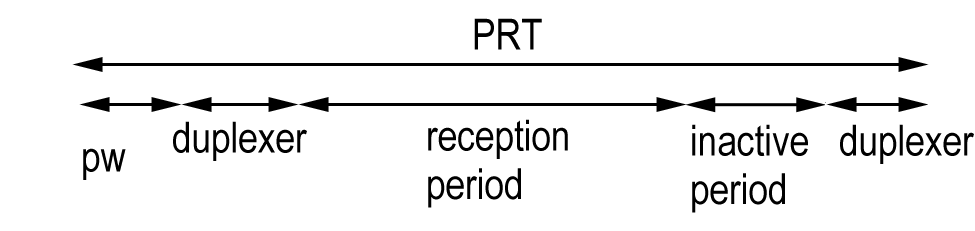
\includegraphics[width=6cm]{timescales.png}
  \caption{\textit{Description of the pulse cycle. PRT, reception period and inactive period has duration in milliseconds, whereas duplexer switch time and pulsewidth are in microseconds.}}
  \label{fig:timescale}
\end{figure}

The earliest time any sampling may occur in any pulse emission cycle is limited by the time switching from emission of reception, here referred to as \textit{duplexer\_switch\_time} and the actual length of the pulse, or \textit{pulse\_width}. The shortest distance from which any signal sampling may originate is:
\begin{equation}
2L_{mininum}=c(t_{duplex} + t_{pulse}) \Rightarrow L_{minimum}=\frac{ c(t_{duplex}+t_{pulse}) }{2}
\end{equation}

By default, the time between each sampling is equal to half the pulsewidth, but may be set to other values as well. The time between each sampling corresponds also to a distance between each sampling. If the time between each samples the signal at time \(t\), the corresponding equation for the distance to target is:
\begin{equation}
2L = ct \Rightarrow L = \frac{ct}{2}
\end{equation}
If the sampling takes place a time \(\Delta t\) later, the corresponding distance is:
\begin{equation}
L' = \frac{c(t + \Delta t)}{2}
\end{equation}
The distance between each sampling is thus:
\begin{equation}
\Delta L = L' - L = \frac{c\Delta t}{2}
\end{equation}

\(\Delta L\) is referred to as the \textit{range bin} distance. 


\section{Unit System}
This library, both C++ and Python, uses a strict SI unit system. Only basic SI unit are used. This means distances are measured in meters only, not km, cm, miles, feet, inches or anything else. There is one exception to basic SI units. This applies to setting up a radar. For setting up a radar, normal conventions apply, such as using microseconds to describe pulsewidths and decibels for describing antennae gain. Once these figures are set, they are treated like basic SI further on, meaning pulsewidth is described in seconds and antennae gain is unitary. 

Angles are described in radians, except for setting up a radar. 

\subsection{Coordinate System}
Input coordinates for any position relevant to the radar, is given in figure \ref{fig:coordinates}. Input coordinates are east, north and zenith for coordinate axes, and azimuth, elevation and distance for spherical coordinates. When treated in the bkradsim library, the corresponding cartesian coordinates are x, y, z, with spherical coordinates \(\theta\), \(\phi\) and \(r\):
\begin{equation}
  x = r \cos{\phi}\cos{\theta}, y = r \cos{\phi}\sin{\theta}, z = r\sin{\phi}
\end{equation}
\begin{figure}
  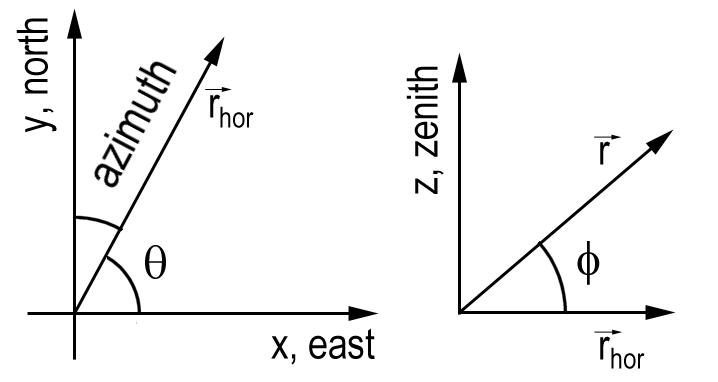
\includegraphics[width=6cm]{axes.png}
  \caption{\textit{Coordinates.}}
  \label{fig:coordinates}
\end{figure}

\subsection{The 'amp' unit}
The strength of received signals is given in power, P, whose unit is watt (W):
\begin{equation}
P = V \times I = \frac{V^{2}}{R} = IR^{2}
\end{equation}
\(V\), \(I\) and \(R\) are voltage, current and resistance, respectively. It is feasible to make a calculution of the received signal pwoer. Unfortunately, one has to handle superposition of signals, making it necessary to handle the signal in voltage or current. BKRadSim does not model any impedance of the electronic system. As workaround, instead of modelling voltage or current, the square root of the power signal will suffice. The unit of is referred to as \(amp=\sqrt{W}\). Adding two signals of power \(P_{a}\) and \(P_{b}\) that are in phase is thus:
\begin{equation}
P_{total}=(Signal_{a} + Signal_{b})^{2}=(\sqrt{P_{a}}+\sqrt{P_{b}})^{2}
\end{equation}

This merely affects the internal signals handling in the library and will usually not affect any user. 



\chapter{C++: installing the library}
This library was made for linux only. It is not Windows compatible. In fact it will not even compile on Windows systems. 
\section{Ubuntu, Debian: installing from terminal}
\lstset { %
    language=bash,
    backgroundcolor=\color{black!5}, % set backgroundcolor
    basicstyle=\footnotesize,% basic font setting
}
This option is not yet available. However, when it will be just write:
\begin{lstlisting}
sudo apt-get install libbkradsim-dev
\end{lstlisting}
\section{Red Hat, Fedora: installing from terminal}
This option is not yet available. However, when it will be just write:
\begin{lstlisting}
yum install libbkradsim-dev
\end{lstlisting}


\chapter{C++ Tutorial}
\lstset { %
    language=C++,
    backgroundcolor=\color{black!5}, % set backgroundcolor
    basicstyle=\footnotesize,% basic font setting
}
\section{Starting to use the library}
The easiest place to start is to see if the compiler can handle the include files. Here is the code for just that:
\begin{lstlisting}
#include <radsim/radar/adc.hpp>

int main() {
    return 0;
}
\end{lstlisting}
The next step is to use one of the BKRadSim-objects - the ADC (Analog to Digital Converter). This is just to assert that you can use the libbrkadsim.so binary file:
\begin{lstlisting}
#include <radsim/radar/adc.hpp>
#include <iostream>

int main() {
    ADC adc(10, ADCMode::Power, 1e-12);
    std::cout << adc.convert(1e99) << std::endl;
    return 0;
}
\end{lstlisting}
The resultant code should print \(1023\) in the terminal. 
\section{Using the Radar class}
\subsection{Generate radar pulses} \label{subsec:gen_pulse}
The following program will perform a simple radar simulation:
\begin{lstlisting}
#include <iostream>
#include <string>
#include <vector>
#include <radsim/radar/radar.hpp>
#include <radsim/radar/radar_config.hpp>
#include <radsim/radar/radar_config_parser.hpp>

using namespace std;
using namespace radsim;

void displayPulseData(const PulseData& pulse_data) {
  auto& reg = pulse_data.registry;
  for (size_t i = 0; i < 10; i++)
    cout << "--- sampling " << i << ": " << reg[i] << endl;
}


int main() {
   RadarConfigParser parser;
   string config_file = "stationary_radar.txt";
   RadarConfig config = parser.parseFile(config_file);
   Radar radar(config);

   cout << "Sim time(s): " << radar.getCurrentTime() << endl;
   auto pulse_data = radar.generatePulseData();
   cout << "Sim time(s): " << radar.getCurrentTime() << endl;
   pulse_data = radar.generatePulseData();
   cout << "Sim time(s): " << radar.getCurrentTime() << endl;
   displayPulseData(pulse_data);
   
   return 0;
}
\end{lstlisting}
The radar configuration file, "stationary\_radar.txt", must be set up as thus:
\begin{verbatim}
Frequency        10.0 #Ghz
PeakPower        10000 #W
PulseWidth       0.25 #microsec
MaxReceiveTime   0.4 #ms
PRT              5000 #ms
BandWidth        4.0 #Mhz
NoiseFigure      4.0 #db
DuplexSwitchTime 3.08333333 #microsec
AntennaeGain     30.0 #db
AzBeamWidth      2.0 #deg
ElBeamWidth      40.0 #deg

ADCResolution    12 #bit
ADCMode          Power
ADCMin2Noise     0.01953125 #unit
\end{verbatim}
The "config.txt" file describes a radar with the above characteristics, and is typical of a maritime navigation radar (except that the navradars typically use a carrier frequency of 9.4 Ghz, they rotate, has a pulse repetition time in the range of milliseconds and have a lower sensitivity). The rotation speed of the antennae is not, set. It is by default zero. The radar points by default along the east axis. 

The execution of the program should produce this result in the terminal:
\lstset { %
    language=bash,
    backgroundcolor=\color{black!5}, % set backgroundcolor
    basicstyle=\footnotesize,% basic font setting
}
\begin{lstlisting}
Sim time(s): 0
Sim time(s): 5
Sim time(s): 10
--- sampling 0: 10
--- sampling 1: 81
--- sampling 2: 49
--- sampling 3: 27
--- sampling 4: 132
--- sampling 5: 7
--- sampling 6: 45
--- sampling 7: 26
--- sampling 8: 2
--- sampling 9: 56
\end{lstlisting}
\lstset { %
    language=C++,
    backgroundcolor=\color{black!5}, % set backgroundcolor
    basicstyle=\footnotesize,% basic font setting
}
The program prints the simulation time before and after the emission of two radar pulses, in addition to the first 10 radar samlings recorded after emission of the second pulse. Multiple executions of the program yields different values and they may appear random. They are. There is no clutter or target in this setup. The only origin of any signal is the internal radar receiver noise. 

The following will explain the code in more detail. 

The \textit{RadarConfigParser} class defines objects used for reading radar configuration files, as in the example with "config.txt" above. It has a default constructor and two public member functions:
\begin{lstlisting}
class RadarConfigParser {
  public:
  RadarConfigParser();
  RadarConfig parseFile(const std::string& config_file) const;
  RadarConfig parseString(const std::string& config_str) const;
};
\end{lstlisting}
These two member functions produce \textit{RadarConfig} objects, which contain the information needed to set up a \textit{Radar} object. 

The \textit{Radar} class is the core of BKRadSim. \textit{Radar} class object does mainly the following:
\begin{enumerate}
\item \textbf{Pulse data generation}: Through the function \textit{generatePulseData}, generates the sampled signals from an emitted pulse and store the in a std::vector container. 
\item \textbf{Simulation time keeping}: The radar keeps track of the simulation time. 
\end{enumerate}
It takes a \textit{RadarConfig} object as argument. In this example and the next, several \textit{Radar} member functios are also used:
\begin{lstlisting}
class Radar {
  public:
  Radar(const RadarConfig& config);
  double getRange(int index) const; //m
  double getCurrentSimTime() const; //s
  PulseData generatePulseData(const Target& target, 
                              bool signal_override = false,
                              double signal_strength = 0);                              
};
\end{lstlisting}
\textit{generatePulseData} takes a pointer to a \textit{Target} objects and returns a \textit{PulseData} object. The function also has two default arguments that are omitted in this example. After creating the \textit{PulseData} object, the simulation clock is advanced to the start of the next emission period. In this example, a NULL object is used for target which means no target information is used. 

The \textit{PulseData} object is the final product of the radar calculations. It contains three important member variables: the time of the emitted pulse, the boresight direction of the antennae and finally a vector containing the sampled signals as converted into discrete (integer) values. This data is enough to start digital processing of the data:
\begin{lstlisting}
class PulseData {
  public:
  std::vector<unsigned short> registry;
  double getStartTime() const; //s
  math_vector getBoresight() const;                      
};
\end{lstlisting}
The \textit{registry} member contains all the signal samplings recorded in the pulse emission period. 

\subsection{Setting up a target}
The \textit{Target} class has two constructors:
\begin{lstlisting}
class Target {
  public:
  Target(math_vector position, double rcs);
  //position: [m, m, m];
  //rcs: m2
  Target(ApproxFunction<math_vector> path, double rcs);
  //path: func(s) = [m, m, m]
  //rcs_: m2
};
\end{lstlisting}
The first constructor takes a position argument, in this case a \textit{math\_vector} class argument. \textit{math\_vector} is just a std::array of size 3, used for denoting 3-dimensional physics vectors: position, speed and acceleration. Using this constructor, we instantiate a motionless target. 

The other argument, \textit{rcs}, is the target radar cross section. 

In order to instantiate a \textit{moving} target, the \textit{Target} constructor needs a 'path' argument instead of a 'position' argument. A path argument is of the type \textit{ApproxFunction}. 
\begin{lstlisting}
template <class T>
class ApproxFunction {
  public:
  ApproxFunction(std::vector<double> entry_, std::vector<T> value);
  T output(double x);
  //t: s                    
};
\end{lstlisting}
T can be either double, std::complex\textless double\textgreater or \textit{math\_vector}. For a path argument, T is a \textit{math\_vector}. The entry variable describes a vector of simulation points in time. The points in time must correspond to a vector of \textit{math\_vector} positions of similar size, that is at time entry[i] the target is located at value[i]. The following defines a path where the target is at 10000 m east at time t = 0 s and moves to 9800 m east at time t = 10 s:
\begin{lstlisting}
ApproxFunction<math_vector> path({0, 10.0}, 
                                 {{10000, 0, 0}, {9800, 0, 0}} );
\end{lstlisting}
The function \textit{output} produces a linear weighted value as function the input x. In the example above, path.output(5.0) would produce the vector [9900, 0, 0].

\subsection{Target detection in the presence of noise}
When the \textit{Radar} is set to add receiver noise to calculations, any positive signal cannot be classified to be of a target origin. There is no support for any digital processing in BKRadSim - the \textit{Radar} class is only meant to supply the digitally sampled raw signal. Any user has to set up the entire digital processing chain him(her)self. For detections in the presence of white noise, there is a simple technique called Constant False Alarm Rate (CFAR). This technique works as follows: on the std::vector registry, \(r\) containing all the sampling per pulse: for each index, a background is created involing the surrounding indices. Since the target usually covers several sampling indices, or \textit{range bins}, the closest indices are not used. We are going to use the following algorithm:
\begin{enumerate}
\item For the first index \(i\):
\item \quad create \(sum\_left = \sum_{j=i-N-b}^{i-b-1}{r_{j}}\)
\item \quad create \(sum\_right = \sum_{j=i+b+1}^{i+b+N}{r_{j}}\)
\item \quad Calculate \(background=(sum\_left + sum\_right) / (2N) \) 
\item \quad Detection is positive if \(r_{i} > T \times background \)
\item When advancing to next index:
\item \quad \(\Delta sum\_left = r_{i-b} - r_{i-N-b}\) 
\item \quad \(\Delta sum\_right = r_{i+b+N+1}-r_{i+b}\)
\item \quad i++
\item \quad Calculate  \(background=(sum\_left + sum\_right) / (2N) \) 
\item \quad Detection is positive if \(r_{i} > T \times background \)
\end{enumerate}
\(b\) range bins on each side of the cell in question are not used due to the fact that a target contributes to more than one range bin due to size, high simpling frequency and bandpass filtering. \(N\) range bins on each side of the cell in question are also used to detect a background. \(T\) is a thresholding parameter. Due to the statistical nature of noise and clutter, a false detection may always occur. The purpose of CFAR is that if the general noise level increases, the detection threshold also increases, thus maintaining a constant rate of false detections (or alarms). If a single pulse signal is used for detection, setting the detection threshold to 14 times the average backround noise (\(T = 14\)) results in a chance of false detection at 1 ppm per range bin \cite{ref:levanon} (pp. 43). In the next section, we will set up this CFAR algorithm with \(N=15, b=3, T=20\).

\subsection{Detection of a moving target} \label{CFAR-program}
Here is an example of a new program using the CFAR detection algorithm on a moving target:
\begin{lstlisting}
#include <iostream>
#include <string>
#include <vector>

#include <radsim/mathematics/math_vector.hpp>
#include <radsim/radar/target.hpp>
#include <radsim/radar/radar.hpp>
#include <radsim/radar/radar_config.hpp>
#include <radsim/radar/radar_config_parser.hpp>

using namespace std;
using namespace radsim;

//Target detection using a CFAR detection algorithm   
double detectTargetDistance(const Radar& radar, 
                           const PulseData& pulse_data,
                           int N, int b, double T) {
  const auto& reg = pulse_data.registry;

  size_t i = N + b;   //minimum range bin to perform CFAR
  size_t i_max = reg.size() - N - b; //max range bin for CFAR

  int sum_left = 0;
  size_t j_min_left = i - N - b;
  size_t j_max_left = i - b;
  for (size_t j = j_min_left ; j < j_max_left; j++)
    sum_left += reg[j];

  int sum_right = 0;
  size_t j_min_right = i + b + 1;
  size_t j_max_right = i + b + N + 1;
  for (size_t j = j_min_right; j < j_max_right; j++)
    sum_right += reg[j];

  int num_bins = 0;
  double sum_range = 0;
  while ( i <= i_max ) {
    double threshold = T * (sum_left + sum_right) / (2.0 * N);
    if (reg[i] > threshold) {
      sum_range += radar.getRange(i); //m
      num_bins++;
    }
    sum_left  += reg[j_max_left]  - reg[j_min_left];
    sum_right += reg[j_max_right] - reg[j_min_right];
    j_min_left++; j_max_left++; j_min_right++; j_max_right++;
    i++;
  }
  return sum_range / (double)num_bins; //m
}


void detectTarget(Radar& radar, const TargetCollection& targets) {
  double t = radar.getCurrentTime();
  auto pulse_data = radar.generatePulseData(targets);  
  double distance = detectTargetDistance(radar, pulse_data, 
                                         15, 3, 22);
  cout << "Time(s): " << t << ", distance(m): " << distance << endl;  
}


int main() {
  ApproxFunction<math_vector> path({0.0, 20.0}, 
                                   {  {0, 10000, 0}, 
                                      {0, 9600, 0}  });

  TargetCollection targets;
  targets.emplace_back(move(path), 50000.0);

  RadarConfigParser parser;
  RadarConfig config = parser.parseFile("stationary_radar.txt");
  Radar radar(config);

  detectTarget(radar, targets);
  detectTarget(radar, targets);
  detectTarget(radar, targets);
  detectTarget(radar, targets);
  detectTarget(radar, targets);
  return 0;
}
\end{lstlisting}
The program should produce the following output:
\lstset { %
    language=bash,
    backgroundcolor=\color{black!5}, % set backgroundcolor
    basicstyle=\footnotesize,% basic font setting
}
\begin{lstlisting}
Time(s): 0, distance(m): 9996.87
Time(s): 5, distance(m): 9912.5
Time(s): 10, distance(m): 9809.37
Time(s): 15, distance(m): 9696.87
Time(s): 20, distance(m): 9612.5
\end{lstlisting}
The target moves exactly 100 m per 5 seconds starting 10000 m north. The output produces a result that is slightly off exact target position. This is due to the total accuracy of the radar setup and digital processing algorithm. 

The function \textit{detectTarget} calls the \textit{Radar} member function \textit{generatePulseData} with a \textit{const Target*} argument. The function \textit{getDistance} uses the CFAR algorithm detailed in the previous chapter. To get range information from a sampling with index i, \textit{Radar::getRange} is called with i as argument. \textit{getDistance} produces a positive result is a target is detected and zero otherwise. 

\section{Using the RadarInterface class}
\subsection{Generate pulses using RadarInterface}
The \textit{RadarInterface} class is used to test processing algorithms in near realtime. The \textit{RadarInterface} class owns a \textit{Radar} class and spawns a thread which run radar simulations in parallell to any digital processing. This is one of the main features of BKRadSim; the signal simulations and digital processing run separately and in parellell. As a consequence a dual core CPU or better is required to use the \textit{RadarInterface} class. 

The following presents code for an initial sample program. It will display the resultant samplings of the first received pulses.

\lstset { %
    language=C++,
    backgroundcolor=\color{black!5}, % set backgroundcolor
    basicstyle=\footnotesize,% basic font setting
}

\begin{lstlisting}
#include <iostream>
#include <string>
#include <vector>
#include <radsim/mathematics/math_vector.hpp>
#include <radsim/radar/target.hpp>
#include <radsim/radar/radar_interface.hpp>
#include <radsim/radar/radar_config.hpp>
#include <radsim/radar/radar_config_parser.hpp>

using namespace std;
using namespace radsim;


int main() {
  RadarConfigParser parser;
  auto config = parser.parseFile("naval_radar.txt");

  TargetCollection targets;
  targets.emplace_back( (math_vector){0, 5000, 0}, 2 );

  RadarInterface radar_if(config, targets);

  radar_if.start();
  int count = 0;
  while (count <= 10) {
    if (radar_if.dataReady()) {
      auto pulse_data = radar_if.getData();

      cout << "t(s): " << pulse_data.getStartTime() << ": ";
      for (size_t i = 250; i < 260; i++)
        cout << pulse_data.registry[i] << ", ";
      cout << endl;

      count++;
    }      
  }
  cout << radar_if.getSimTime();
  radar_if.stop();

  return 0;
}
\end{lstlisting}
The configuration file "naval\_radar.txt" must be set up as thus. 
\begin{verbatim}
#This is a radar config for a general navigation radar
#Receives detections up to 60 km. 

Frequency        9.4 #Ghz
PeakPower        10000 #W
PulseWidth       0.25 #microsec
PRT              2.0 #ms
MaxReceiveTime   0.4 #ms
BandWidth        4.0 #Mhz
NoiseFigure      4.0 #db
DuplexSwitchTime 1.0 #microsec
AntennaeGain     30.0 #db
AzBeamWidth      2.0 #deg
ElBeamWidth      40.0 #deg
AntRotationSpeed 180.0 #deg/s, clockwise rotation

ADCResolution    14 #bit
ADCMode          Power
ADCMin2Noise     0.1 #unit
\end{verbatim}
There are changes compared to the previous config file. Firstly, the pulse repetition time is 2 ms, not 5000 ms. There is also a rotation speed: 180 degrees pr second, or 2 s pr full rotation (scan time). The rotation speed is set by keyword "AntRotationSpeed". 
The ADC resoultion (keyword "ADCResolution") is 14-bit, and the sensitivity (keyword "ADCMin2Noise") is set higher. 

Instead of a \textit{Radar} object, a \textit{RadarInterface} object is initiated:
\begin{lstlisting}
class RadarInterface {

   private:
   Radar radar;

   public:
   RadarInterface(const RadarConfig& config, 
                  list<Target> targets, 
                  double dt = 0.15);

   void start(bool signal_override = false, 
              double signal_strength = 0);

   void stop();    
   double getSimTime() const; //s

   bool dataReady();
   PulseData getData();
};
\end{lstlisting}
Like a \textit{Radar} object, the constructor takes a config file and a list of targets. The last construction variable, dt, is optional and is the minimum time before any simulation time update (in seconds). The simulation time is updated after each pulse generation and the set minimum time, \textit{dt}. Simulation time is accessed via the function \textit{getSimTime}. A private \textit{Radar} class object is where all calculations takes place. Invoking \textit{start} spawns a thread in which the simulator runs. The \textit{Radar} object will then continuously generate \textit{PulseData} objects, by repeated call of the fucntion \textit{Radar::generatePulseData}. These \textit{PulseData} objects are one-by-one inserted into a queue called the data-queue. In order to get objects from the data-queue, two functions are necessary. \textit{dataReady} tells if there are any objects available. \textit{getData} extracts and returns one \textit{PulseData} object from the queue. Note: attempting to extract when the queue is empty will result in an exception.  

The function \textit{stop} stops and destroys the thread and any objects associated with it.
 
Running the program, the printout in the terminal window should look like this (the values are random, so do not expect an exact outcome):
\lstset { %
    language=bash,
    backgroundcolor=\color{black!5}, % set backgroundcolor
    basicstyle=\footnotesize,% basic font setting
}
\begin{lstlisting}
t(s): 0: 1, 2, 14, 5, 21, 3, 20, 3, 5, 25, 27, 7, 4, 27, 1, 
t(s): 0.002: 4, 30, 5, 4, 0, 3, 3, 2, 9, 9, 29, 3, 2, 24, 6, 
t(s): 0.004: 16, 1, 40, 11, 22, 14, 5, 17, 8, 2, 45, 20, 0, 0, 5, 
t(s): 0.006: 1, 14, 2, 14, 5, 6, 12, 14, 2, 3, 0, 11, 2, 4, 30, 
t(s): 0.008: 22, 31, 4, 5, 3, 13, 25, 8, 1, 8, 10, 38, 22, 14, 10, 
t(s): 0.01: 13, 0, 17, 11, 0, 1, 4, 4, 12, 2, 6, 6, 0, 0, 5, 
t(s): 0.012: 5, 5, 21, 9, 25, 2, 10, 2, 9, 18, 0, 11, 24, 12, 7, 
t(s): 0.014: 10, 22, 9, 24, 2, 8, 5, 19, 3, 15, 3, 6, 2, 2, 12, 
t(s): 0.016: 12, 13, 14, 1, 4, 0, 1, 2, 9, 15, 3, 1, 13, 6, 5, 
t(s): 0.018: 11, 10, 0, 8, 9, 7, 16, 42, 11, 15, 12, 3, 18, 9, 1, 
t(s): 0.02: 5, 0, 8, 13, 0, 2, 6, 3, 3, 0, 2, 7, 41, 9, 2, 
\end{lstlisting}
The printout displays the first 15 signal samplings of the first 11 pulses along with a start time for each pulse emission. The results are produced on average every 2 ms. As you might expect, the sampled signals are random and originate from noise. The target is actually located further out, near rangebin 257. If we were to change the code slightly by displaying range bins 250 to 260 instead, the result would be different:
\begin{lstlisting}
t(s): 0: 2, 2, 2, 9, 29, 3, 245, 1991, 2418, 690, 
t(s): 0.002: 0, 4, 27, 6, 11, 4, 132, 1722, 2006, 533, 
t(s): 0.004: 1, 1, 21, 3, 29, 18, 169, 870, 1362, 225, 
t(s): 0.006: 10, 6, 7, 3, 1, 5, 6, 452, 496, 107, 
t(s): 0.008: 12, 29, 3, 16, 14, 51, 12, 126, 108, 13, 
t(s): 0.01: 13, 0, 2, 0, 4, 5, 22, 39, 52, 23, 
t(s): 0.012: 8, 1, 3, 28, 0, 11, 0, 0, 10, 17, 
t(s): 0.014: 0, 19, 1, 0, 0, 0, 7, 2, 15, 32, 
t(s): 0.016: 0, 8, 29, 0, 7, 19, 3, 10, 15, 7, 
t(s): 0.018: 0, 8, 20, 0, 11, 12, 25, 20, 1, 17, 
t(s): 0.02: 45, 18, 1, 5, 16, 2, 7, 2, 9, 4, 
\end{lstlisting}
In addition to the many small random numbers, a cluster of high numbers also appear. That cluster of high numbers originate from the target. The first line originates when the radar is pointing directly at the target. For the consequent pulses, the antenna is increasingly pointing away from the target, and therefore the target contribution starts to fade away. As seen in figure \ref{fig:det_cluster}, the signals are clustered around a target, and any 2D per-scan detection algorithm need to take this into account. 

\begin{figure}
  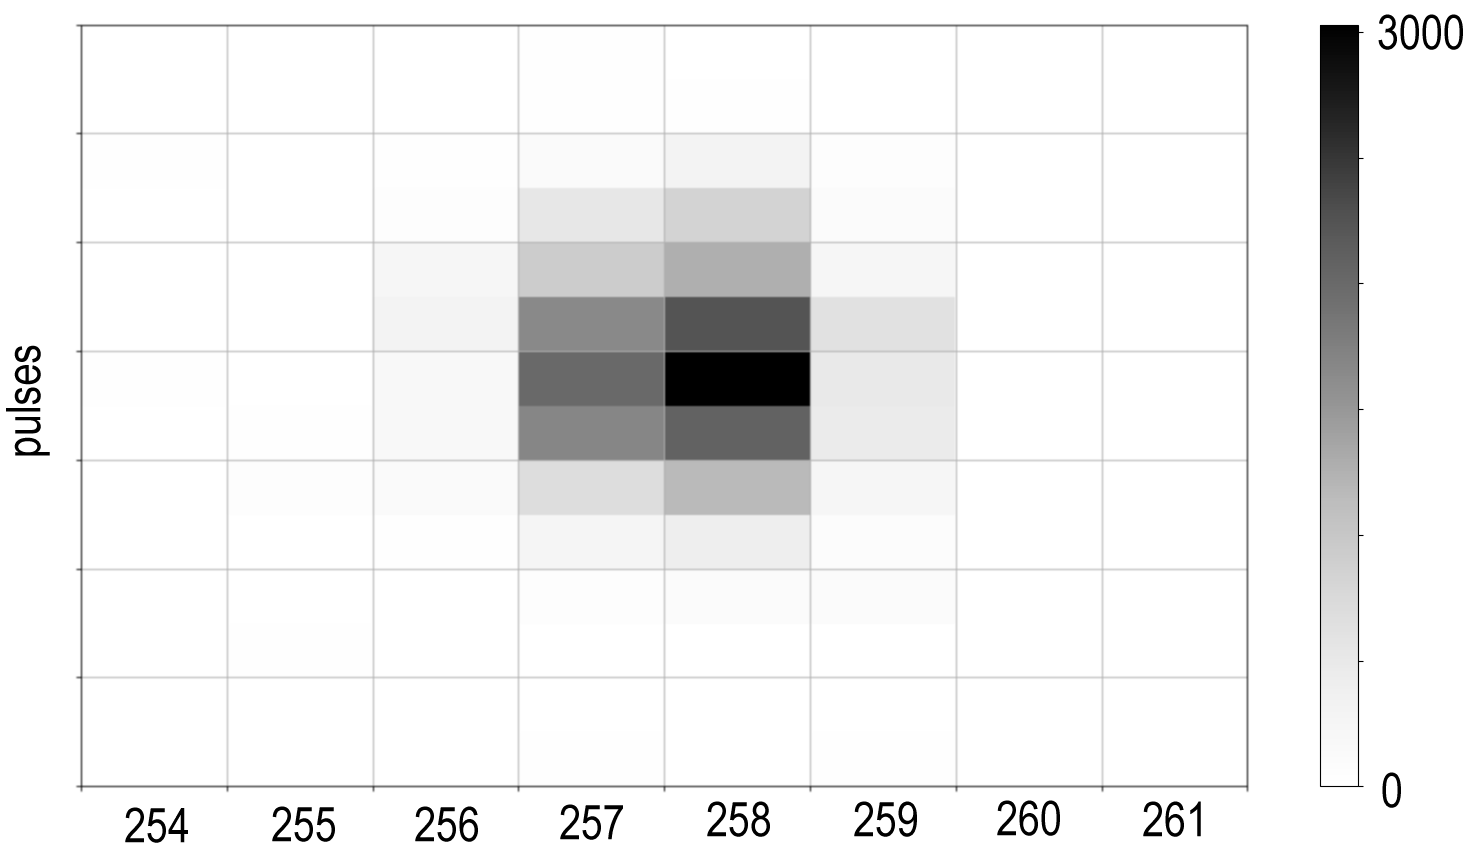
\includegraphics[width=6cm]{det_cluster.png}
  \caption{\textit{Signal measurements produced when a radar beam sweeps by a target.}}
  \label{fig:det_cluster}
\end{figure}


\subsection{2D plot formation}
With a rotating antenna supplying measurement data in both distance and azimuth, two dimensional target position data can be generated. As seen in the previous subsection, the signal from one target does not result in a substantial signal in a single CUT, but rather a cluster of strong signals. Similarly, applying CFAR will also result in clusters of detections. Hereafter, we are going to refer to CFAR detections as \textit{raw detections}. What we need is to treat a bunch of raw detections as one detection, or \textit{plot}. 

The algorithm is very simple: We keep a record of the clusters that are under development. When processing a pulse, raw detections are grouped into clusters in the radial direction, called \textit{linear clusters}. If any of these linear clusters are in the vicinity of any of the clusters in the record, we will update that cluster. Otherwise, a new cluster is added to the record. After going through the raw detections, we iterate the record of clusters. Any cluster without update is considered finished, erased from the record and is transformed into a plot. Obviously, this needs a bit of coding. The entire code is in the file 'processor.cpp'. It is a bit long for adding into a text document, but the main points will be outlined. 

First. we create the \textit{Cluster} class itself. Also, a struct for the linear clusters in the radial direction, called \textit{LinearCluster}, is created:
\begin{lstlisting}
struct LinearCluster {
  int weight;
  math_vector pos; //[m, m, m]
  double time; //s

  LinearCluster(double t, int w, const math_vector& p) :
    time(t), weight(w), pos(p)
  {}
};

class Cluster {
  private:
    int bin_min;
    bool updated;
    vector<LinearCluster> rad_clusters;

  public:
    Cluster(int bin_min_arg, int bin_max_arg, 
            double t, const math_vector& pos_arg) 
    {
      update(bin_min_arg, bin_max_arg, t, pos_arg);    
    }

    int getMin();
    bool isUpdated();
    void reset();
    void update(int bin_min_arg, int bin_max_arg, 
                double t, const math_vector& pos_arg);
    void printPlot();
};
\end{lstlisting}

\textit{LinearCluster} onws three parameters: the pulse time, \textit{time}, the number of detections in the radial cluster, \textit{weight} and lastly the average position as determined form the range bin indices. The \textit{Cluster} class constructor takes 4 arguments. \textit{bin\_min\_arg} and \textit{bin\_max\_arg} the the detection range indices for the first and last detection for the linear cluster. The \textit{update} funciton is called at construction and each time there is pulse-data to update the cluster. At construction, or update, a LinearCluster is added to its private list. When there is no update for the cluster, \textit{printPlot} then uses info from its list of \textit{LinearClusters} to find a mean position in space and time. That position is the plot, and for this program it is just printed in the terminal. 

The \textit{DigitalProcessor} class is created to control the simulation. It owns a \textit{RadarInterface} instance, and the settings for clustering and CFAR. The record of clusters exist as a std::list Cluster instance. 
\begin{lstlisting}
class DigitalProcessor {
  private:
  RadarInterface radar;

  //CFAR parameters:
  int N = 20;  //number of samples at each side of CUT
  int b = 3;   //closest cells to CUT not used for threshold
  double T = 30;  //Thresholding parameter

  //Clustering parameters:
  int tolerance = 2;
  list<Cluster> clusters;

  vector<int> generateRawDetections__(const PulseData& pulse_data);
  list<Cluster>::iterator findCluster__(int bin_min);
  void handleCluster__(const PulseData& pulse_data, 
                         int cl_min, int cl_max);
  void updateClusters__(const PulseData& pulse_data, 
                          const vector<int>& detections);
  void processPulse__();
  void generatePlots__();

  public:
  DigitalProcessor(RadarConfig& config, TargetCollection targets)
    : radar(config, move(targets))
  {}

    void generate(double max_time);
};
\end{lstlisting}
The function \textit{generate} is the only public function. Invoking it will make the radar run a certain time, \textit{max\_time}, and process the continous stream of data into plots, which are then displayed on the screen. 
\begin{lstlisting}
void DigitalProcessor::generate(double max_time) {
  radar.start();

  while (radar.getSimTime() < max_time)
    if (radar.dataReady()) processPulse__();

  radar.stop();
}
\end{lstlisting}
\textit{generate} starts the radar, then go in a continous loop until a certain time has passed. When any PulseData object is ready for in the \textit{data queue}, it is then processed in the function \textit{processPulse\_\_}:
\begin{lstlisting}
void DigitalProcessor::processPulse__() {
  auto pulse_data = radar.getData();
  auto detections = generateRawDetections__(pulse_data);
  updateClusters__(pulse_data, detections);
  generatePlots__();
}
\end{lstlisting}


\textit{updateClusters\_\_} separates the raw detections into linear clusters. Each separation invokes a call to \textit{handleCluster\_\_} which again either creates a new cluster, or updates a cluster whose rangebin indices are close by.
The last part of the process is the function \textit{generatePlots\_\_}, which checks which plots are updated and creating plots from and erases those that are not.

The 'main' function of the program is finally set up as follows:
\begin{lstlisting}
int main() {

  TargetCollection targets;
  targets.emplace_back( (math_vector){0, 5000, 0}, 50 ); 

  RadarConfigParser parser;
  auto config = parser.parseFile("naval_radar.txt");

  DigitalProcessor processor(config, move(targets));
  processor.generate(10.0);

  return 0;
}
\end{lstlisting}
A target are generated as input to the DigitalProcessor. We use the same 'naval\_radar.txt' setup as before. When executing the program, the result should look somewhat like this:
\lstset { %
    language=bash,
    backgroundcolor=\color{black!5}, % set backgroundcolor
    basicstyle=\footnotesize,% basic font setting
}
\begin{lstlisting}
25: Plot pos: [69.0588, 5016.24], t = 0.00438095
25: Plot pos: [3.21375, 5015.52], t = 2.00021
25: Plot pos: [-1.98925e-09, 5016.3], t = 4
25: Plot pos: [-3.8641, 5015.43], t = 5.99976
25: Plot pos: [3.21375, 5015.52], t = 8.00021
25: Plot pos: [-7.87403e-09, 5016.3], t = 10
25: Plot pos: [-3.21375, 5015.52], t = 11.9998
25: Plot pos: [-4.25, 5016.64], t = 13.9997
\end{lstlisting}
The target is located North, and a plot will appear almost instantly after the simulated radar beam sweeps by the North position every 2nd second, provided adequately fast computer. Since the processes are statistically based, running the program several times might result in some plots originating from noise, but most of the time the outpout will be clean. This particular setup is actually well tuned, and does not represent a typical per-scan processing output. Typically, the thresholding parameter \(T\) is lowered for the benefit of higher detection probability. Setting to a lower value, say \(T = 12\), will result in many more detections. Running it for 0.5 seconds \, we get: 
\begin{lstlisting}
Plot pos: [3.39265e-12, 55406.2], t = 0       <-- False
Plot pos: [75.3144, 5013.56], t = 0.00478261  <-- True
Plot pos: [2570.92, 27197.5], t = 0.03        <-- False
Plot pos: [17106.5, 49456.3], t = 0.106       <-- False
Plot pos: [7456.47, 20711.1], t = 0.11        <-- False
Plot pos: [2451.38, 3706.44], t = 0.186       <-- False
Plot pos: [15588.9, 6059.06], t = 0.382       <-- False
Plot pos: [10831.9, 3899.72], t = 0.39        <-- False
Plot pos: [9536.1, 3231.5], t = 0.396         <-- False 
Plot pos: [2040.48, -115.51], t = 0.518       <-- False
\end{lstlisting}
Most of the plots are false, i.e. originating from noise. An interesting feature can be seen if we set up the target as moving and plot several scans in two dimensions. The target is in this case set up as such, moving in the south direction:

\lstset { %
    language=C++,
    backgroundcolor=\color{black!5}, % set backgroundcolor
    basicstyle=\footnotesize,% basic font setting
}
\begin{lstlisting}
  ApproxFunction<math_vector> path ( {0, 30}, { {0, 5000, 0},
                                                {0, 4400, 0} } );

  TargetCollection targets;
  targets.emplace_back( move(path), 50 );
\end{lstlisting}
In figure \ref{fig:multiple_scans} we have plotted the results from 30 seconds of rotation. Most of the plots can be seen as random noise. However, those originating from the target form a pattern, a line. This is a way to visualize the radar output. Plot from a single scan is meaningless, unless the detection threshold is very high and we are dealing with high signature targets. Therefore, in order to successfully carry out area surveillance, information form several scans is nescessary. 

\begin{figure}
  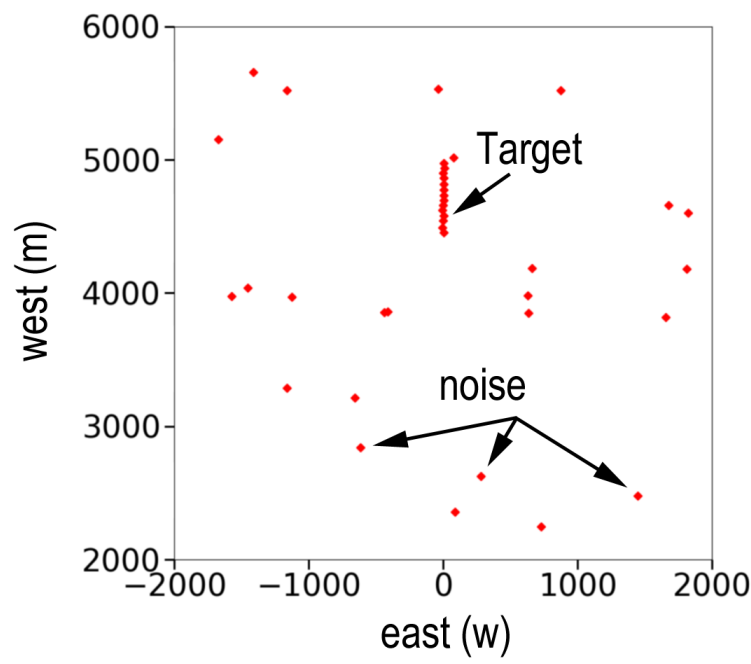
\includegraphics[width=6cm]{plot_scans.png}
  \caption{\textit{Radar plots in the course of 15 radar scans over 30 minutes.}}
  \label{fig:multiple_scans}
\end{figure}


\subsection{Notes on Tracking}
As seen, in order to provide dynamic and cleaner output, the processing need to take into account the signals from more than one radar scan. Plot visualization using several radar scans is a way to do it, but it can also be done automatically. This is \textit{track processing}. The challenges of a track algorithms is not to loose opportunities to detect a target, not to create false tracks in a cluttered or multi-target environment, and maintaining an establish track. In order for the track algorithm to be deemed successful, all this need to work in realtime and with multiple targets.

With regards to dynamic data, kalman filtering or the method of least squares can be applied. The difficult part is track initiation. In this case, the algorithm must perform as a classifier, picking plots or raw signals assosiated with a suspected real target and disregarding the rest. As an example procedure track algorithm, the reader may attempt a simple technique that should work for the detection of boats: 

A class \textit{Track} should be created, with structure and members
\begin{itemize}
\item A queue storing the last 3 plot updates.
\item A projected dynamic model of the path of the target based on previous target positions. This could simply be a linear model using the method of least squares, or a path model based on Kalman filtering.
\item A function that provides a gate. The gate is an area where new plots can used to update the track. At creation time this should be a square with sides \(a = 2 \times scantime \times v_{max}\). \(v_{max}\) is the expected maximum speed of a target. \(v_{max} = 20m/s\) should suffice for boats, save professional racers. When the track as been updated several times, this gate shoule be smaller as it is easier to predict the future track position. The centre of the gate is determined by the dynamic model. 
\end{itemize}

The iterative procedure is a follows: 
\begin{itemize}
\item When a new plot is present, attempt to associate it with present tracks. The plot should have a timestamp \(t\). For each track, calculate its present position. Center the track gate on that position, then check if the plot is in that position. If so, that plot is used to update the track. The plot is stored in the queue and used to update the dynamic model of the track. The track should be marked as updated until the next scan. 
\item If the plot cannot update a track, then a new tentatve track is created. 
\item a check should be created: if the track is tentative, drop it if it missed updates the following to scans after initiation (it is called a 3 out of 3 algorithm), otherwise elevate status to ordinary track. Drop any track tracks altogether if they have not been updated in 7 radar scans.
\end{itemize}

There are two main track initiation algorithms: batch and sequential. In the sequential approach, each scan is processed while available to the tracker. The logical type of initiation, which is the algorithm presented above, is a subtype in which a tentative track is asserted based on N out of M updates \cite{ref:bar-shalom_et_al, ref:xi_et_al}. Another sequential approach, introduced in \cite{ref:hough} is the Sequential Probability Ratio Probability (SPRT) method, where a likelihood (score) is calculated for each track candidate at each time stamp. A likelihood test is then applied to decide wether a target is present or not. 

In batch processing, several scans are processed together. One such technique is the Hough transform \cite{ref:hough} where imperfect instances of objects, such as lines, can be found in a high clutter environment. The Hough transform work well in environments with high false alarm rates, but may find tracking initiation difficult where there are deviations from expected target paths.

In addition to these more determininst approaches, machine learning should be studied. This includes neural networks for batch processing of radar scans, or self-learning clustering algorithms to automatically detect patterns. Of interest would be to completely bypass the CFAR algorithm, with the possibility of higher detection probability with yet a reduced false alarm rate. Many scientific papers have already been published about this \cite{ref:justin_et_al}. When applied to real time processing, the algorithms are of couse finished trained and thus adjusted for what they are intended for. The heavily vectorized calculations may still require a lot of computing power. Many desktop computer are equipped with graphics cards, and it might be an idea to use them for this purpose as they are ideally suited for the linear algebra associated with neural networks. Although used for training the algorithm, instead of continuous processing, Guo et al. \cite{ref:guo_et_al} use this for a sea clutter suppression algorithm. 




\chapter{C++ Library Documentation}
\section{Mathematics}

\lstset { %
    language=C++,
    backgroundcolor=\color{black!5}, % set backgroundcolor
    basicstyle=\footnotesize,% basic font setting
}
\subsection{ApproxFunction}
Include statement:
\begin{lstlisting}
#include <radsim/mathematics/approx_function.hpp>
\end{lstlisting}
Class prototype:
\begin{lstlisting}
template <class T>
class ApproxFunction {

public:
  ApproxFunction(T value_);
  ApproxFunction(std::vector<double> entry, 
                 std::vector<T> value);
  ApproxFunction(std::vector<double> entry, 
                 std::vector<T> value, 
                 T initial_value, T end_value);

  T output(double x) const;
  std::vector<T> outputVector(std::vector<double> input) const;
  const std::vector<double>& getEntryVector() const;
  const std::vector<T>& getValueVector() const;
};
\end{lstlisting}
An \textit{ApproxFunction} is a class representation of a linearly interpolated approximation of a function. Supposing a function \(G(x)\), calculate two series of values, \(x_{i}\) and \(G_{i}\) such that:
\begin{equation} \label{eq:ApproxFunction}
g_{i} = G(x_{i})
\end{equation}
The different values \(x_{i}\) are evenly spaced, where \(x_{i+1} - x_{i} = Constant = \Delta x\). G(t) can be approximated by:
\begin{equation} \label{eq:ApproxOutput}
G \approx w_{n} \times g_{n+1} + w_{n-1} \times g_{i}
\end{equation}
\begin{equation}
n = floor{((t - x_{0}) / {\Delta x})} + 1
\end{equation}
\begin{equation}
w_{n} = (x_{i} - t) / {\Delta x}
\end{equation}
\begin{equation}
w_{n-1} = (t - x_{n-1}) / {\Delta x}
\end{equation}
T may be either double, std::complex$\langle$double$\rangle$, or math\_vector. The values of \textit{entry} need to be equally spaced. The first constructor produces an \textit{ApproxFunction} with constant value output. The second and third constructor produces an output represented by equation \ref{eq:ApproxOutput}. 

\textit{output} produces the result of equation \ref{eq:ApproxOutput}. If the input \textit{x} is outside the range of the constructur argument \textit{entry}, the output will be:
\begin{itemize}
\item Having used the second constructor, the output will be the endpoint of the constructur argument \textit{value}.
\item Having used the third constructor, the output will be either \textit{initial\_value} or \textit{end\_value}. 
\end{itemize}
\textit{outputVector} produces a vector of outputs by invoking \textit{output} for each value in \textit{input}. 

Example constant function:
\begin{lstlisting}
ApproxFunction<double> g(12);
\end{lstlisting}
\begin{equation}
g(x) = 12
\end{equation}

Example triangular step function:
\begin{lstlisting}
ApproxFunction<double> g({0, 1}, {0, 1});
\end{lstlisting}
\begin{equation}
g(x) = \begin{cases} 
          0 & x < 0 \\
          x & x \in [0, 1> \\
          1 & x \geq 1 
       \end{cases}
\end{equation}

Example square function:
\begin{lstlisting}
ApproxFunction<double> g({0, 1}, {1, 1}, 0, 0);
\end{lstlisting}
\begin{equation}
g(x) = \begin{cases} 
          0 & x < 0 \\
          1 & x \in [0, 1> \\
          0 & x \geq 1 
       \end{cases}
\end{equation}


\subsection{mathutils}
Include statement:
\begin{lstlisting}
#include <radsim/mathematics/mathutils.hpp>
\end{lstlisting}
Function prototypes:
\begin{lstlisting}
double rayleighPDF(double x_avg, double Q); //unit as [x_avg]
       //x_avg: var
       //Q: [0, 1>, input to PDF from random number generator

double powerToAmp(double power); //amp
       //Power: W

void  setRadDefaultRange(double& theta); //theta set in 
                                         //range [0, 2pi>
     //theta: rad
\end{lstlisting}
\textit{rayleighPDF}: Random input in the range \(Q \in [0, 1> \) and with an average ouput of \(x_{avg}\) produces an output with distribution:
\begin{equation}
p(x) = \frac{1}{x_{avg}}\exp{(-x)}
\end{equation}
\textit{powerToAmp} converts signal value from power to amplitude:
\begin{equation}
amplitude = \sqrt{power}
\end{equation}
\textit{setRadDefaultRange}:
\begin{equation}
\theta = \theta_{0} + 2 \pi n \rightarrow \theta_{0}, \quad \theta_{0} \in [0, 2\pi>
\end{equation}




\subsection{math\_vector}
Include statement:
\begin{lstlisting}
#include <radsim/mathematics/math_vector.hpp>
\end{lstlisting}

Class definition and functions prototypes:
\begin{lstlisting}
typedef std::array<double, 3> math_vector;

//scalar product
double      operator * (const math_vector& a, const math_vector& b);

//vector times scalar
math_vector operator * (const math_vector& a, double c);
math_vector operator * (double c, const math_vector& a);
math_vector operator / (const math_vector& v, double s);
void operator /= (math_vector& a, double c);
void operator *= (math_vector& a, double c);

//vector addition
math_vector operator + (const math_vector& a, const math_vector& b);
math_vector operator - (const math_vector& a, const math_vector& b);

double      math_vector_length(const math_vector& v);
double      math_vector_angle(const math_vector& a, 
                              const math_vector& b); //rad
math_vector math_vector_unit(const math_vector& v);
std::string to_string(const math_vector& v);
void        math_vector_set_unit(math_vector& v);
bool        math_vector_equal(const math_vector& a, 
                              const math_vector& b, 
                              double relative_error); 
\end{lstlisting}
The \textit{math\_vector} is used to describe 3-dimensional physics variables. Included in library are some functions for handling vector calculus. 


\section{Radar}

\subsection{ADC}
Include statement:
\begin{lstlisting}
#include <radsim/radar/adc.hpp>
\end{lstlisting}
Class prototype:
\begin{lstlisting}

enum class ADCMode { Power, Logarithm };

class ADC
{
  public:
  ADC(int resolution, ADCMode mode, 
      double min_power, double max_power = 0);
  //resolution: bit
  //min_power: W
  //max_power: W

  int getNumLevels() const;
  double getSensitivity() const; //W

  unsigned short convertSignal(double amplitude) const; //unit
  //Amplitude: amp
};
\end{lstlisting}
The analog to digital converter, or ADC, handles conversion of received signal into digital - integer - values. The settings for Power and Voltage are minimum and maximum power, \(P_{min}\) and \(P_{max}\) and number of possible levels, \(N\) possible to measure up to 16bit. Signals stronger than the maximum will have value \(N-1\). For Power mode, the maximum power setting is irrelevant. The equations for the digititzed measurements are \ref{eq:ADC_Power} and \ref{eq:ADC_Logarithmic} for power and logarithmic mode, respectively.
\begin{equation} \label{eq:ADC_Power}
I=\begin{cases}
      floor{\frac{p}{P_{min}}} & p < P_{max} \\
      N-1 & p \geq P_{Max}
   \end{cases}
\end{equation}
\begin{equation} \label{eq:ADC_Logarithmic}
I=\begin{cases}
      0 & p < P_{min} \\
      floor(C \log{\frac{p}{P_{min}}}) & P_{min} < p < P_{max} \\
      N-1 & p \geq P_{Max}
   \end{cases}, C=\frac{N-1}{\log{P_{max} / P_{min}}}
\end{equation}

Example initiate 8-bit ADC in power mode, with sensitivity \(10^{-14}\) W. 
\begin{lstlisting}
ADC adc(256, ADCMode::Power, 1e-14);
\end{lstlisting}

Example initiate 10-bit ADC in logarithmic mode, with sensitivity \(10^{-14}\) W. 
\begin{lstlisting}
ADC adc(1024, ADCMode::Logarithm, 1e-14, 1e-12);
\end{lstlisting}

The function \textit{getSensitivity} returns \(P_{min}\). 

The function \textit{convertSignal} takes a value in 'amp' units (not W!) and converts these into an integer measurement.

\subsection{BandpassFilter}
Include statement:
\begin{lstlisting}
#include <radsim/radar/bandpass_filter.hpp>
\end{lstlisting}
Function prototypes:
\begin{lstlisting}
enum class BandpassFilter{Standard, Rectangular};

//func(hz) = unit
ApproxFunction<std::comples<double>> 
createBandpassFilter(BandpassFilter type, double bandwidth);
//bandwidth: hz
\end{lstlisting}
\textit{createBandPassFilter} returns an \textit{ApproxFunction} object which is normally used in the bandpass filter equation, eq. \ref{eq:signal_reception_0} and setting of average receiver noise level, equation \ref{eq:noise_power}. Currently, there are two predefined filters which are selected by the \textit{type} argument. One filter is a rectangular filter. The \textit{BandpassFilter::Standard} filter is described in equation \ref{eq:standardfilter} and is shown in figure \textit{fig::standardfilter}. 

\begin{equation} \label{eq:standardfilter}
H(f) = \begin{cases} 
          0 & |f| > \frac{5}{4}bw \\
          \frac{1}{2}{(1-\cos{ ( \frac{\pi(|f|-\frac{5}{4}bw}{\frac{1}{2}bw} ) })} & \frac{3}{4} \geq |f| \leq \frac{5}{4}bw \\
          1 & |f| < \frac{3}{4}bw 
       \end{cases}
\end{equation}
\begin{figure}
  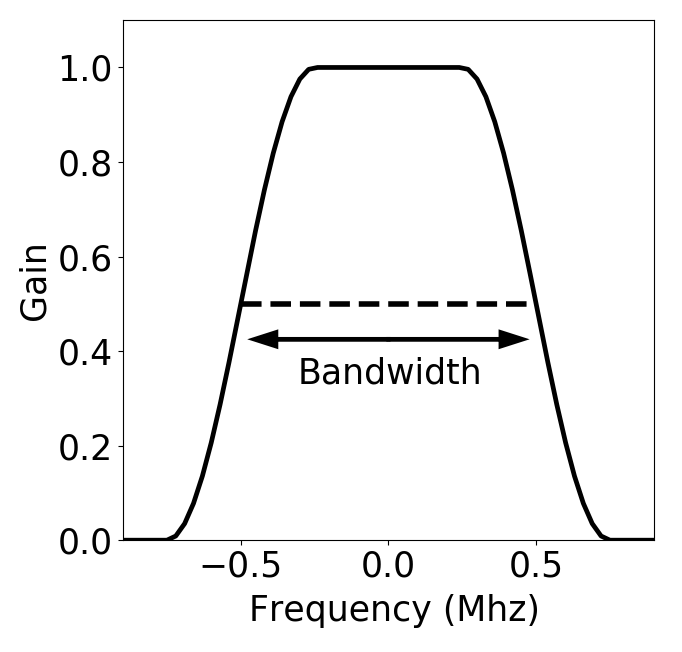
\includegraphics[width=6cm]{BandPassFilter.png}
  \caption{\textit{The bandpassfilter as defined in equation \ref{eq:standardfilter}, with a bandwidth of 1 Mhz.}}
  \label{fig:standardfilter}
\end{figure}

\subsection{BeamPattern}
Include statement:
\begin{lstlisting}
#include <radsim/radar/beam_pattern.hpp>
\end{lstlisting}
Prototypes:
\begin{lstlisting}
enum class BeamPattern{Triangular, Gaussian};

ApproxFunction<double> createBeamPattern(BeamPattern Shape, 
                                         double beamwidth);
//beamwidth: rad
\end{lstlisting}
\textit{createBeamPattern} returns an ApproxFunction with a particular shape, mimicking the radar beam pattern with a certain beamwidth. The Triangular shape has been added for test purposes. 

\subsection{PulseData}
Include statement:
\begin{lstlisting}
#include <radsim/radar/pulse_data.hpp>
\end{lstlisting}
Include statement:
\begin{lstlisting}
class PulseData {
  public:
  PulseData(double t, math_vector boresight_arg, 
                      std::vector<unsigned short> registry_arg);

  std::vector<unsigned short> registry;
  double      getStartTime() const; //s
  math_vector getBoresight() const; //[unit, unit, unit]
};
\end{lstlisting}
\textit{PulseData} stores the necessary information to carry out digital processing. \textit{registry} contains all signal measurements in one pulse cycle. \textit{getStartTime} returns the time when the pulse started to emit, i.e. the start of the pulse cycle as described in figure \ref{fig:timescale}. \textit{getBoresight} returns a cartiesian vector representing the pointing direction at the start of the pulse cycle. 

\subsection{Radar}
Include statement:
\begin{lstlisting}
#include <radsim/radar/radar.hpp>
\end{lstlisting}
Class prototype:
\begin{lstlisting}
class Radar 
{
  public:
  Radar(const RadarConfig& Config);  

  double getMinimumRange() const; //m, minimum signal detection lim
  double getUnAmbiguousRange() const; //m
  double getRangeBin() const; //m
  double getPeakPower() const; //W
  double getAvgNoise() const; //W
  double getPulseWidth() const; //s
  double getPRT() const; //s
  double getDuplexerSwitchTime() const; //s
  double getSamplingTime() const; //s, time between samplings
  double getMaximumReiceiveTime() const; //s, upper limit time where
                                         //signal sampling may occur
  double getMinimumReceiveTime() const; //s, time, lower limit where
                                        //signal sampling may occur
  double getInitialHorTheta() const; //rad, gets the initial 
                                     //     horizontal position of 
                                     //     the antenna after reset 
                                     //     or before any
                                     //     pulse generation


  double getRange(int bin_index) const; //m, the sampling range 
                                        //corresponding to bin_index.

  bool   getToAddNoise() const;
  bool   getToAddTarget() const;
  bool   getUsePdf() const; //if no, only avg values are used

  ADC getADC() const;

  //func(s) = unit, on amp level
  DoubleApproxFunction getFilteredPulse() const;

  //func(rad) = unit, on power level
  DoubleApproxFunction getHorizontalBeamShape() const;

  //func(rad) = unit, on power level
  DoubleApproxFunction getElevationBeamShape() const;

  void setAntRotSpeed(double w);
  //w: rad/s

  void setToAddNoise(bool set);
  void setToAddTarget(bool set);
  void setUsePdf(bool set); /if no, only avg values are used
  void setToUseFilteredPulse(bool set);

  void setInitialHorTheta(double theta_arg); 
  //theta_arg: rad

  const math_vector& getCurrentBoresight() const;
  double getCurrentTime() const; //s
  PulseData generatePulseData(const vector<Target>& targets, 
                              bool signal_override = false, 
                              double signal_strength = 0);
  void reset(double t = 0);
  //t: s
};
\end{lstlisting}
The \textit{Radar} class is responsible for running the simulation. It keeps track of the simulated time, and produces signal measurements delivered in the form of \textit{PulseData} containers. 

The constructor takes a \textit{RadarConfig} argument containing all the necessary settings. Note that the constructor calls \textit{RadarConfig::assertParametersSet} to check for logical inconsistencies or neglected mandatory parameters. Please refer to the table in subsection \ref{chap:radar_config}. If the check fails, an exception is thrown. 

\textit{Radar::generatePulseData} is the most import function, delivering signal measurement data. For each range bin, a combined signal of receiver noise and target echo is calculated. How this is done, is described in chapter \ref{chap:physical_model}. This function changes the state of simulation. After each invokation of \textit{generatePulseData}, the current time and the current position of the antennae is set to the start of the next pulse emission cycle. Detections beyond unambiguous range are also stored and will be handled when \textit{generatePulseData} is invoked next. If \textit{signal\_override} is set to \textbf{true}, the power of the received echo is not calculated as in chapter \ref{chap:physical_model}, but is instead set by argument \textit{signal\_strength}. 

\textit{Radar::reset} sets the Radar to a start position at time \(t\). The antenna is set to the start position. 


\subsection{RadarConfig}
\label{chap:radar_config}
Include statement:
\begin{lstlisting}
#include <radsim/radar/radar_config.hpp>
\end{lstlisting}
Class prototype:
\begin{lstlisting}
class RadarConfig {

  public:
  RadarConfig();

  void assertParametersSet() const;

  void setPeakPower(double power);
  //Power: W

  void setFrequency(double f);
  //f: Ghz

  void setPulseWidth(double pulsewidth);
  //pulsewidth: microsec

  void setSamplingTime(double samplingtime);
  //sampligtime: microsec

  void setPRT(double t);
  //t: ms

  void setMaximumReceiveTime(double t);
  //t: ms

  void setBandWidth(double bandWidth);
  //bandWidth: Mhz

  void setNoiseFigure(double noiseFigure);
  //noiseFigure: db, since this is regarded as more front-end.
    
  void setDuplexerSwitchTime(double switchTime);
  //switchTime: microsec   

  void setAntennaeGain(double gain);
  //gain: dB

  void setAzBeamWidth(double horizontalBeamWidth);
  //horizontalBeamWidth: //degrees, NOT rad

  void setElBeamWidth(double elevationBeamWidth);
  //horizontalBeamWidth: //degrees, NOT rad

  void setAntennaeRotationSpeed(double speed);
  //speed: degrees/s

  void setAzimuth(double azimuth);
  //azimuth: deg

  void setHorizontalBeamShape(BeamPattern pattern) {
    horizontal_beam_shape = pattern;
  }

  void setElevationBeamShape(BeamPattern pattern) {
    elevation_beam_shape = pattern;
  }

  void setADCMode(ADCMode adcMode);
  void setADCResolution(unsigned int resolution);

  void setADCMax2Noise(double ratio);
  //ratio: unit

  void setADCMin2Noise(double ratio);
  //ratio: unit

  double getPeakPower() const; //W
  double getFrequency() const; //hz
  double getPulseWidth() const; //s
  double getSamplingTime() const; //s
  double getPRT() const; //s
  double getMaximumReceiveTime() const; //s
  double getBandWidth() const; //hz
  double getNoiseFigure() const; //unit, NOT db
  double getDuplexerSwitchTime() const; //s
  double getAntennaeGain() const; //unit
  double getHorizontalBeamWidth() const; // rad
  double getElevationBeamWidth() const; // rad
  double getAntennaeRotationSpeed() const; // rad/s
  double getTheta() const; // rad

  BeamPattern     getHorizontalBeamShape() const;
  BeamPattern     getElevationBeamShape() const;
  ADCMode         getADCMode() const;
  unsigned int    getADCResolution() const;
  double          getADCMax2Noise() const; //unit
  double          getADCMin2Noise() const; //unit  
};
\end{lstlisting}
The \textit{RadarConfig} takes all necessary parameters to set up a \textit{Radar} class instance. Note that while the BKRadSim library uses primarily basic-SI units, the \textit{set} functions \textit{RadarConfig} takes values in units typically used for describing radars. The \textit{get} functions returns basic-SI. 

The function \textit{RadarConfig::assertParametersSet} is used to check that all mandatory parameters are set. This function also checks for logical inconsistencies. If all mandatory parameters are not set, or a logical inconsistency is found, an exception is thrown. The \textit{Radar} class always invokes this function during construction in order to avoid problems during subsequent execution. The parameters are:

\begin{center}
\begin{tabular}{ p{5em} p{2em} p{12em} p{8em} } 
 paramater & unit & description & default value \\
 \hline
 frequency & Ghz & carrier frequency of emitted pulse &  - - - \\ 
 peak power & W & pulse power during emission & - - - \\
 pulsewidth (pw) & \(\mu\)s & timelength of pulse & - - - \\
 pulse repetition time (PRT) & ms & pulse repetition time &  - - - \\
 maximum reception time & ms & upper limit time after emission start where signal reception is possible & \(PRT - dswitch\) \\
 sampling time & \(\mu\)s & time between each signal measurement & \(\frac{1}{2}pw\) \\
 duplexer switch time (dswitch) & \(\mu\)s & the time is takes to switch from emission to reception or vice versa & - - - \\
 bandwidth & Mhz & width of bandpass filter at recepction &  - - - \\
 antennae gain & db & the gain of the antenna & - - - \\
 horizontal beamwidh & \(^{o}\) & half width of beam in the horizontal plane & - - - \\
 vertical beamwidh & \(^{o}\) & half width of beam in the vertical plane & - - - \\
 antenna rotation speed & \(^{o}/s\) & speed is positive in the clockwise direction around the compass & \(0^{o}/s\) \\
 azimuth & \(^{o}\) & the azimuth pointing direction of antenna at start & \(0^{o}\), north \\
 ADC resolution & bit & any value from 1 up and including 16. & - - -\\
 ADC mode & string & the ADC can be either in power or log mode & - - -\\
 ADCMin2 Noise & unit & measure of sensitivity, i.e. sensitivity is \(ADCMin2Noise \times avgnoise\) & - - -\\
 ADCMax2 Noise & unit & in log mode, max power is \(ADCMax2Noise \times avgnoise\) & - - -\\
\end{tabular}
\end{center}
Only non-mandatory parameters have default values. 


\subsection{RadarConfigParser}
Include statement:
\begin{lstlisting}
#include <radsim/radar/radar_config_parser.hpp>
\end{lstlisting}
Class prototype:
\begin{lstlisting}
class RadarConfigParser {
  public:
  RadarConfigParser();
  RadarConfig parseFile(const std::string& filename) const;
  RadarConfig parseString(const std::string& config_string) const;
};
\end{lstlisting}
The role of the \textit{RadarConfigParser} is to convert a radar configuration in text format to a \textit{RadarConfig} instance which again can be used to set up a \textit{Radar} instance. \textit{parseString} takes input in the form of a string, and \textit{parseFile} reads a file. The output of both functions is a \textit{RadarConfig} instance. 

Example, reading a configuration file called "config.txt":
\begin{lstlisting}
RadarConfigParser parser;
RadarConfig = parser.parseFile("config.txt");
\end{lstlisting}

Example, reading a text string:
\begin{lstlisting}
const string config_str = string { R"(
  Frequency        10.0 #Ghz
  PeakPower        10000.0 #W
  PulseWidth       0.25 #microsec
  PRT              2.0 #ms
  BandWidth        4.0 #Mhz
  NoiseFigure      4.0 #db
  DuplexSwitchTime 500.0 #microsec
  AntennaeGain     30.0 #db
  AzBeamWidth      2.0 #deg
  ElBeamWidth      20.0 #deg

  ADCResolution    1024 #integer
  ADCMode          Power
  ADCMin2Noise     0.01953125 #unit
  )"};
RadarConfigParser parser;
RadarConfig = parser.parseFile(config_str);
\end{lstlisting}
The structure of a radar config file is described in chapter \ref{chap:configfile}.


\subsection{RadarInterface}
\label{chap:RadarInterace}
Include statement:
\begin{lstlisting}
#include <radsim/radar/radar_interface.hpp>
\end{lstlisting}
Class prototype:
\begin{lstlisting}
class RadarInterface {

  private:
  Radar radar
  TargetCollection collection

  public:
  RadarInterface(const RadarConfig& config, 
                       TargetCollection target_collection, 
                       double dt = 0.15);
  //dt: s, timestep in the simulation, before updating sim_time. 

  void setStatistics(bool set);
  //set: if true, A printout of how much simulator thread worked, 
  //is printed. Default set = false

  void setAddNoise(bool set);
  //set: if yes: radar receiver noise is added to simulation.
  //default: true

  void start(bool signal_override = false, 
             double signal_strength = 0);
  //signal_override: if yes, then 
  //received signal is signal_strength.

  void stop();
    
  double getSimTime() const; //s
  bool dataReady();
  PulseData getData();
  double getRange(int bin_index); //m

};
\end{lstlisting}
The \textit{RadarInterface} class owns a \textit{Radar} instance where calls to \textit{Radar::generatePulseData} is run in parallell to the main thread. The constructor takes three arguments. The first is the \textit{RadarConfig} instance used to construct the private \textit{Radar} class instance. The next argument is a \textit{TargetCollection}, or rather std::list of type \textit{Target}. Note that this is not a reference parameter. A user has a choice of either let a \textit{TargetCollection} be copied or to use the std::move function to let the interface class take ownership of it. The constructor parameter \textit{dt} is a measure for often the common time parameter between the main and radar thread is updated. 

\textit{start} starts the simulator. The functions has two defaults arguments, and are the same arguments passed to the invokation of \textit{Radar::generatePulseData}. \textit{generatePulseData} is called repeteadly, and will push \textit{PulseData} objects into a buffer. This will continue endlessly until the function \textit{stop} is called. 

\textit{dataReady} returns \textbf{true} if data is available in the buffer and \textbf{false} if not. If there is data in the buffer, one \textit{PulseData} object can be retrieved at a time, by invoking \textit{getData}. Note that calling \textit{getData} while the buffer is emtpy will result in an exception. 

\textit{setStatistics} will give a printout of how much time the simulator thread has spent working. If too close to 100 percent or above, the simulator will just work slower, but it will not fail. 

\textit{getSimTime} will return the time as kept by the \textit{Radar} object. This time is updated after each period \textit{dt} and at elast one pulse cycle. 


\subsection{Target}
Include statement:
\begin{lstlisting}
#include <radsim/radar/target.hpp>
\end{lstlisting}
Class prototype:
\begin{lstlisting}
class Target
{
  public:
  Target(const math_vector& pos, double rcs);
  //x: m
  //rcs: m2

  Target(ApproxFunction<math_vector>, double rcs);
  //path: func(s) = [m, m, m]
  //rcs_: m2

  math_vector getPosition(double t = 0) const; //m
  //t: s, time position along path curve

  //func(s) = [m, m, m]
  const VectorApproxFunction& getPath() const;

  double getRCS() const; //m2

  void setPosition(const math_vector& pos);
  //pos: [m, m, m]
};
\end{lstlisting}
The \textit{Target} class contains the information necessary to describe a radar target. There are two constructor, the first is used to initiate a fixed position target. The second constructor is used to initiate a moving target, using a path instead of position argument. The function \textit{getPosition} returns the position the target will be at time t. 

Example fixed position target:
\begin{lstlisting}
Target target({100, 0, 0}, 1.0);
\end{lstlisting}
\begin{equation}
position(t) = [100, 0, 0]
\end{equation}

Example moving target:
\begin{lstlisting}
ApproxFunction<math_vector> path( {0, 10, 20}, { {0, 0, 0}, 
                                                 {100, 0, 0},
                                                 {100, 100, 0} } );
Target target(move(path), 1.0);
\end{lstlisting}
\begin{equation}
position(t) = \begin{cases} 
                 [0, 0, 0] & t < 0 \\
                 [10t, 0, 0] & t \in [0, 10> \\
                 [100, 10(t-10), 0] & t \in [10, 20>  \\
                 [100, 100, 0] & t \geq 20
              \end{cases}
\end{equation}


\chapter{Python}
\lstset { %
    language=Python,
    backgroundcolor=\color{black!5}, % set backgroundcolor
    basicstyle=\footnotesize,% basic font setting
}
At this point, there is no well defined Python library - it is in the making. A present example of library code is this:
\begin{lstlisting}
import numpy as np
from bkradsim.radar import RadarConfigParser, Radar, Target

RadarConfigParser parser;
config = parser("config.txt")
Target target(np.array([10000, 0, 0]), 1.0)
radar = Radar(config)
\end{lstlisting}

The library is intented firstly to mimick the C++ library. There may be, in time, functionality that allows easy data-feed compatible with powerful machine learning libraries.


\chapter{Radar Configuration Files}
\label{chap:configfile}
The radar configuration files are text files holding the necessary information to describe a radar in BKRadSim. A configuration files holds a number of keywords. Each keyword is followed by a value either double, integer or string. The use of the sign '\#' enables commenting. The keywords are:

\begin{itemize}
\item \textbf{Frequency:} The carrier frequency. Unit: Ghz
\item \textbf{PeakPower:} Power during emission: Unit: W
\item \textbf{PulseWidth:} Unit: \(\mu\) s
\item \textbf{PRT:} Pulse Repetition Time. Unit: ms
\item \textbf{MaxReceiveTime:} Time after emission start that the radar is in reception mode. Unit: ms
\item \textbf{NoiseFigure:} Unit: db
\item \textbf{DuplexSwitchTime:} Time lost switching from emission to reception or vice versa. Unit: \(\mu\) s
\item \textbf{AntennaGain:} Unit: db
\item \textbf{AzBeamWidth:} Horizontal beamwidth. Unit: degrees
\item \textbf{ElBeamWidth:} Elevation beamwidth. Unit: degrees
\item \textbf{AntRotSpeed:} The rotation speed in clockwise direction. Unit: degrees/s
\item \textbf{Azimuth:} The initial azimuth pointing direction of the antennae. Unit: degrees
\item \textbf{ADCResoluition:} Bit resolution of analog to digital converter. 10bit = 1024 levels. Unit: bit
\item \textbf{ADCMode:} Type of conversion. Unit: string, possible values: 'Power', 'Logarithm'.
\item \textbf{ADCMin2Noise:} Used for setting the sensitivity, e.g. the minimum measure received power. \(Sensitivity = ADCMin2Noise \times (average noise power)\). Unit: unit. 
\item \textbf{ADCMax2Noise:} Used for setting the sensitivity, e.g. the maximum measure received power. \(Max Power = ADCMax2Noise \times (average noise power)\). Unit: unit. 
\end{itemize}

\chapter{Physical Model}
\label{chap:physical_model}
\section{Radiowave propagation}

\subsection{Radar Equation}
In vacuum, the received power of a radar signal reflected from any target is;
\begin{equation}\label{eq:radar}
P_{received} = \frac{P_{peak}G^{2}\sigma\lambda^{2}}{(4\pi)^{3}R^{4}}
\end{equation}
\(P_{received}\) is received power, \(P_{peak}\) the pulse power during emission, \(G\) is the antennae gain, \(\sigma\) is the radar cross section, \(\lambda\) is the carrier wavelength and \(R\) is the distance to target (\cite{ref:levanon} p. 5). Eq. \ref{eq:radar} also assumes that the target is in boresight. Because of the \(R^{4}\) dependency, the resultant received power is a very weak signal usually in the range of \(10^{-10}\)W to \(10^{-14}\)W. 

\subsection{Antenna Pattern}
If a target is off boresight:
\begin{equation}
G = G_{0}^{2} \times G_{receive} \times G_{emit}
\end{equation}
Where \(G_{0}\) is the gain in boresight, and \(G_{receive}\) and \(G_{emit}\) are modulations due to angle offset. Both \(G_{receive}\) and \(G_{emit}\) are described by the same formulae:
\begin{equation}
G_{receive/emit} = G_{mod}(\phi, \theta)
\end{equation}
Where \(\phi\) and \(\theta\) are the angular spherical coordinates of the target relative to the antenna frame. These coordinates may be different in emission and reception (the antenna may move after emission start). The current model assumes that \(G_{mod}(\phi, \theta)\) can be written:
\begin{equation}
G_{mod}(\phi, \theta) = G_{elevation}(\phi) \times G_{azimuth}(\theta)
\end{equation}
This allows for setting up elevation and azimuth beam pattern separately. Figure \ref{fig:beam_deviation} shows the measured signal from a target moving in a demi-circle centered on the radar. With a beamwidth of 2 degrees, the half width of the Gaussian funnction is about 1.4 degrees due to the multiplied reception/emission effect.

\begin{figure}
  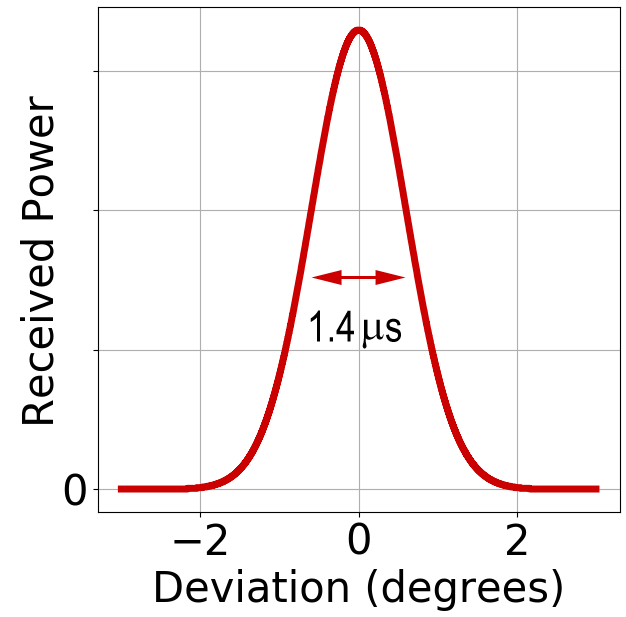
\includegraphics[width=4.5cm]{Dev_Boresight_b.png}
  \caption{\textit{Received signal power from a target as function of boresight deviation. Beamwidth is 2 degrees.}}
  \label{fig:beam_deviation}
\end{figure}

Note on the calculation of angle offset: For calculation purposes, the target and antenna are considered stationary during the pulse emission cycle. As the PRT is on the order of milliseconds, even supersonic targets have movement less than a meter. This is usually far less than the spatial accuracy of most radar systems. For fast rotating antennae, say of 360 degrees per second, 1 millisecond results in a rotation of 0.36 degrees. This may actually have an impact on very accurate systems, and should be taken into account in a future version of the library. If the pulse is received in the next emission cycle, the antennae position is used for the start of that cycle. In that case \(G_{receive} \neq G_{emit}\). 

\section{Signal Reception}
After pulse emission, the radar duplexer swithces from emission to reception mode. There is a minimum wait time before a signal can be sampled, due to pulsewidth and duplexer switch time, \(t_{min}\). The signal will be amplified, after which radar signal of 1 to 40 Ghz is usually mixed down to the IR stage (~60 Mhz) for easier handling. The next stage is the bandpass filtering, followed by the sampling stage where the signal strength is stored in a registry - one such registry for each pulse emitted. 

\subsection{Receiver Noise}
In addition to an incoming signal, thermal noise is introduced in the amplification stage. The level of this noise is:
\begin{equation} \label{eq:noise_power}
N_{avg} = FKT_{E}\int_{-\infty}^{\infty}{|H(f)|^{2}df}=N_{0}\int_{-\infty}^{\infty}{|H(f)|^{2}df}
\end{equation}
\(F\) is the noise figure, usually 2-5 dB, \(K\) is the Boltzmann's constant and \(T_{E}\) is the temperature in Kelvin. \(N_{0}\) is called the spectral noise density. For a rectangular bandpass filter, \(N_{avg}=N_{0}f_{B}\). The noise is random and has a Rayleigh probability distribution function (pdf): 
\begin{equation} \label{eq:Rayleigh_pdf}
p(x) = \frac{1}{N_{avg}} \exp{  - \frac{x}{N_{avg}}   }  
\end{equation}

\begin{figure}
  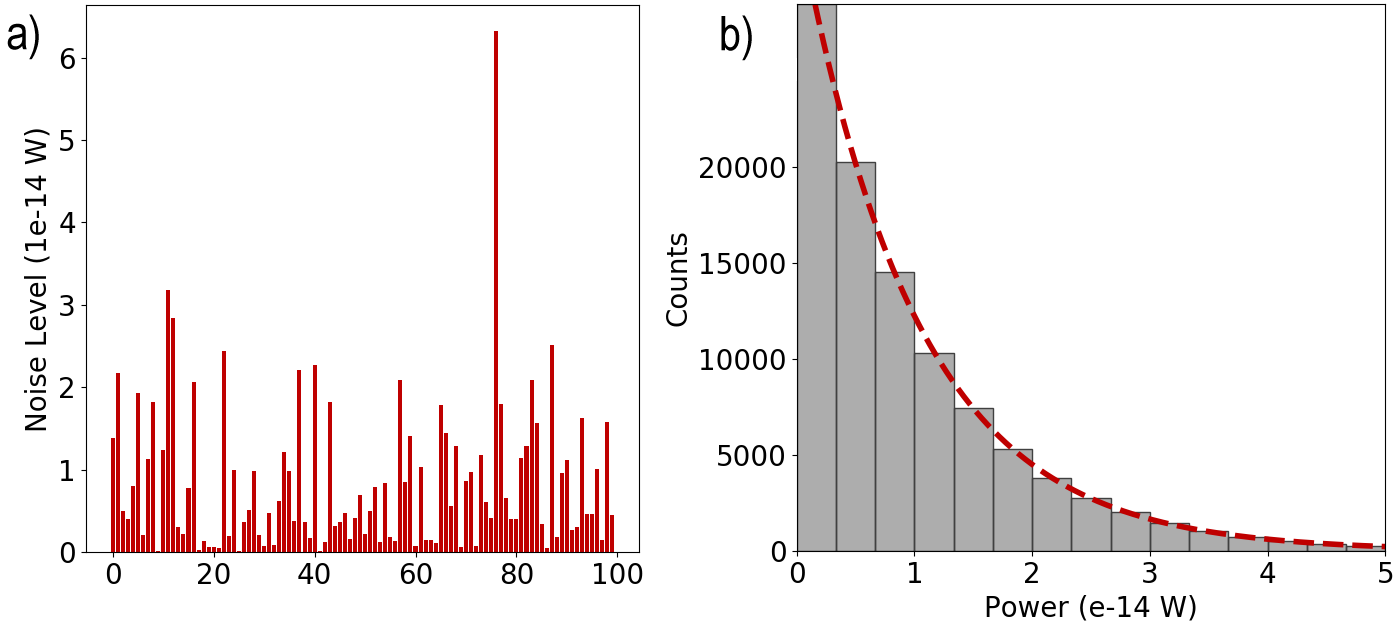
\includegraphics[width=10.5cm]{noise_rayleigh.png}
  \caption{\textit{a) Simator output from a single pulse with no target or clutter, shows receiver noise. b) Histogram showing the power distribution from a Rayleigh distribution. Red line shows the result from equation \ref{eq:Rayleigh_pdf}.}}
  \label{fig:beam_deviation}
\end{figure}

\subsection{Bandpass Filtering of Target Signals}
If the incoming signal is of the form \(s(t)=\sqrt{SignalPower(t)}\), the output from the filter, \(H(f)\) is:

\begin{equation} \label{eq:signal_reception_0}
s_{0}(t) = Fourier^{-1}(S(f)H(f))
\end{equation}

\begin{equation} \label{eq:signal_reception_1}
S = Fourier(s(t))
\end{equation}
BKSimRad will simulate signal filtering as if it was mixed down to zero. If no custom or other predefined filters are selected, BKRadSim will by default use a standard filter as defined in equation \ref{eq:standardfilter}. The filter is displayed in figure \ref{fig:standardfilter}. It is similar to a rectangular filter, but with some tapering at the edges. The typical emitted radar signal would be a pulse of rectangular modulation. For an example below, a pulsetime of \(\tau=1\mu s\) is used. From radar literature  \cite{ref:levanon}, p. 101-106, the ideal bandwidth is close to the inverse of the pulsewidth. In figure \ref{fig:filtered_pulse}, the incoming and the 1 Mhz bandwidth filtered pulse of a \(1\mu s\) signal are displayed. 
The resulting filtered pulse has more of a Gaussian look with extra sidelobes. The amplitude is also lower. The smeared-out shape and lower amplitude is caused by the rather slim bandwidth, not accepting the entire frequency spectrum of the pulse. Choosing a wider bandwith would result in a more square-like shape and a higher amplitude. However, due to radar noise from the amplifier, this is not entirely diserable because, as per equation \ref{eq:noise_power}, a wider bandwidth results in a higher noise level. 

Figure \ref{fig:variable_bandwidth} displays signal power to noise as function of bandwidth. The factor \(q=\frac{bandwidth}{1/\tau}\) is used as a measure of bandwidth. Starting with a slim bandwidth, \(q=0.5\), and increasing it to \(q=1.25\), the signal to noise ratio increases. Increasing from \(q=1.25\) to \(q=2.0\), the signal to noise ratio decreases due to a higher intake of noise through the filter. For \(q=4.0\) the filtered pulse clearly start to appear similar to a rectangular pulse, but the signal to noise ratio is drastically reduced. The most desirable value of \(q\) will vary upon the filter. For a rectangular filter, the ideal value is \(q=1.4\) (\cite{ref:levanon} p. 106). 
\begin{figure}
  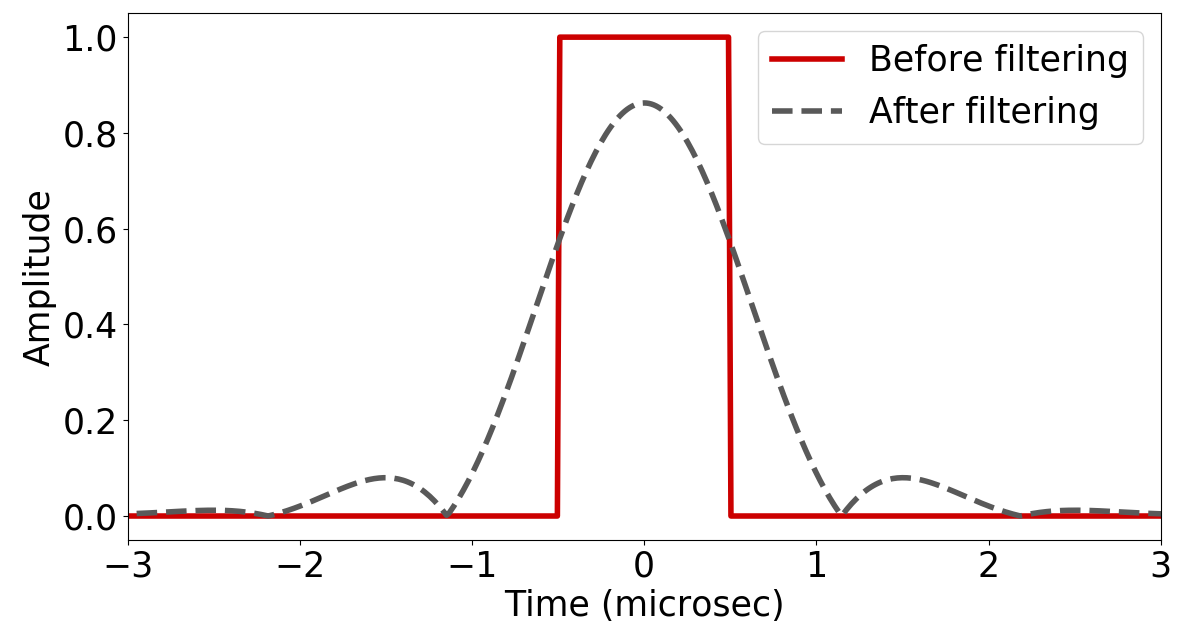
\includegraphics[width=10cm]{PulseFiltering.png}
  \caption{\textit{Incoming square pulse signal of 1\(\mu s\) before and after filtering through a 1 Mhz bandpass filter.}}
  \label{fig:filtered_pulse}
\end{figure}
\begin{figure}
  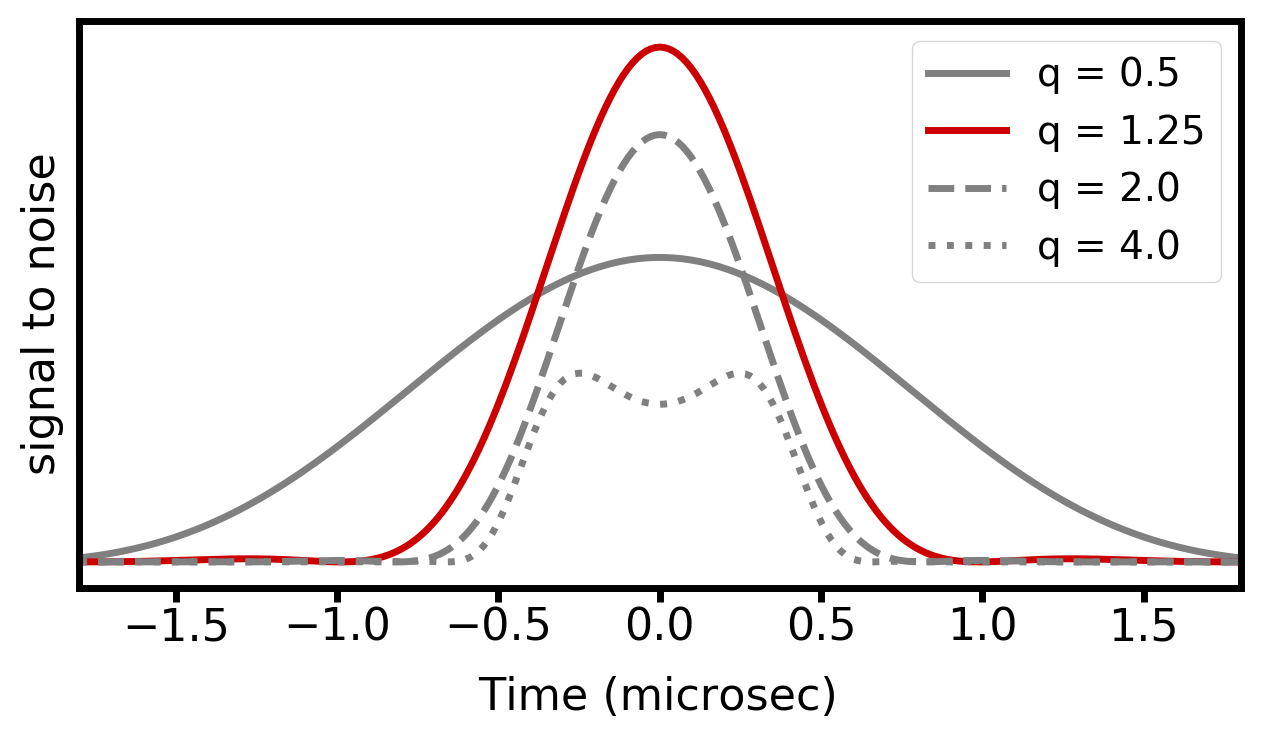
\includegraphics[width=10cm]{VariableBandwith.png}
  \caption{\textit{Signal (power) to noise as function of time for a square pulse incoming signal of duration \(\tau=1\mu s\) for different filter bandwidths using the standardfilter. As a measure of bandwidth, the ratio \(q = \frac{bandwidth}{1/\tau}\) is used.}}
  \label{fig:variable_bandwidth}
\end{figure}

\subsection{Signal Strength at Sampling Stage}
\begin{figure}
  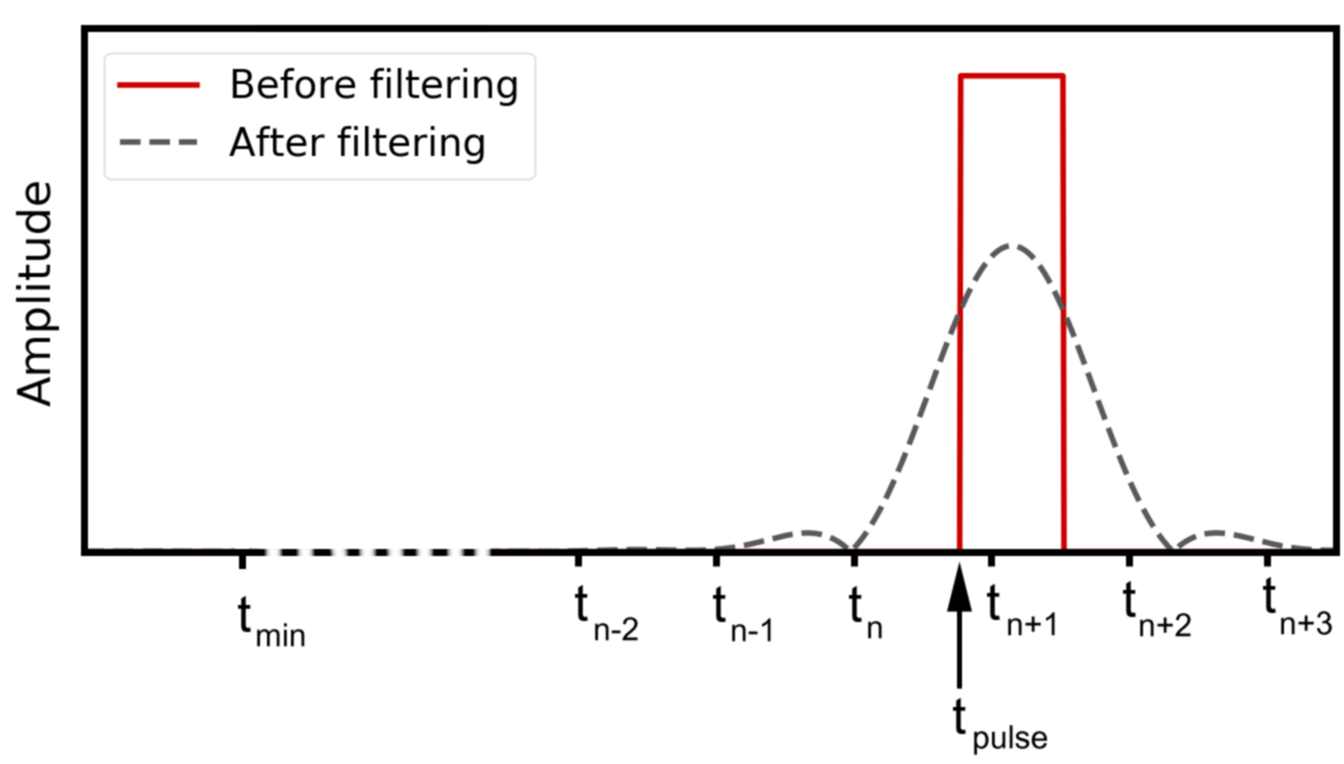
\includegraphics[width=10cm]{Samplings.png}
  \caption{\textit{Sampling of a filtered pulse. \(t_{pulse}\) is the arrival time of the filtered pulse. \(t_{n}\) are sample times.}}
  \label{fig:samplings}
\end{figure}
The individual contributions to signal strength consists of amplifier noise, reflections from target and environment(clutter). These are added at amplitude level:
\begin{equation} \label{eq:total_signal}
\Psi_{total} = A_{target}\exp{\pi i\theta_{target}} + A_{noise}\exp{\pi i\theta_{noise}} + A_{clutter}\exp{\pi i\theta_{clutter}}
\end{equation}
\(\theta_{i}\) denotes an arbitrary angle. \(A_{i}\) is the amplitude of each contributon, i. The sampling of a target signal is calculated as below. Figure \ref{fig:samplings} illustrates the sampling process. A rectangular pulse reflecting from a target at distance \(L\) arrives at time \(t_{pulse}=\frac{2L}{c}\). Due to filtering, the signal will have the shape \(s_{0}(t-t_{pulse})\). As seen in figure \ref{fig:samplings}, samplings are taken at regular intervals, \(\Delta t\), to be digitally sampled and stored in the range bin registry. The target contribution would be:
\begin{equation}
A_{n} = s_{0}(t_{n}-t_{pulse})=s_{0}(t_{min}+n\Delta t-t_{pulse})
\end{equation}
To limit calculation, target contributios can be carried out for:
\begin{equation}
n\in[n_{pulse}-m, n_{pulse}+m+1]
\end{equation}
\begin{equation}
n_{pulse}=floor(\frac{t_{min}-t_{pulse}}{\Delta t})
\end{equation}
\begin{equation}
m=floor{(\frac{3\tau}{\Delta t})}
\end{equation}

\subsection{Beyond Unambiguous Range}
The unambiguous range is given by:
\begin{equation}
L_{amb}=\frac{cT}{2}
\end{equation}
Where \(T\) is the PRT. In case a target is beyond this range in period \(m\), reception will possibly be in the next reception period, \(m+1\). In that case, it is treated in the period \(m+1\) with reception time:
\begin{equation}
t_{pulse}'=t_{pulse}-T
\end{equation}
In case \(t_{pulse}' > T\), reception is possibly in period m+2, in which a reception time \(t_{pulse}''\) is calculated and so on. figure \ref{fig:ambiguous} shows output of a 4 pulse burst. The unambiguous range is 20 km, whereas the target is located a distance of 50 km. In such a case, it is not possible to detect the target in neither pulse 1 nor 2. It is, however detected half-way in the range bin registries of pulse 3 and 4. 
\begin{figure}
  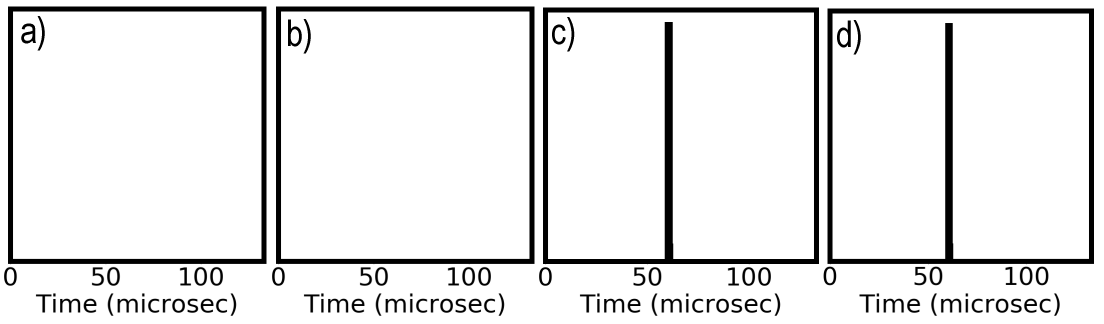
\includegraphics[width=10cm]{ambiguous_montage.png}
  \caption{\textit{Bar histograms showing the range bin registries of a 4 pulse burst in which the target is located a distance of 2.5 times the unambiguous range. a, b, c and d are pulses 1, 2, 3 and 4, respectively.}}
  \label{fig:ambiguous}
\end{figure}


\chapter{Future Development}

Currently BKRadSim has a very simple physical model. However there are some very specific plans for future development: 
\subsection{Sea Clutter Model}
Radio signal backscatter from sea, or \textit{sea clutter} represents a serious problem for most maritime radar systems. Small targets may get obscured by powerful and unpredictable backscattering from the ocean surface. The randomness is more complicated than the white gaussian noise originating in the radar receiver. The clutter has been described \cite{ref:skolnik} (pp. 437) as a speckle part much like white gaussian noise, and \textit{sea spikes} - sporadic signals of high intensity signals with duration in the order of seconds \cite{ref:hansen_et_al}. 

\subsection{Advanced Propagation}
When a pulse signal is emitted from the radar, one part of the signal travels directly and hits a target. Another, emitting from a slightly different angle, reflects from the ocean surface before travelling to the target \cite{ref:skolnik} (pp.239). The latter beam is nearly phase inverted when reflected. Since these beams are close to antiphase, they will almost cancel each other out, significantly shortening the detection distance \cite{ref:levanon} (pp. 77). This is called multipath propagation and is another serious problem with maritime radar detection - more so than the earth curvature. Also, the refraction index changes with height \cite{ref:levanon} (pp 6). From 20m above sea level, it will most consistently decrease. This causes a slight bending of the propagating beam towards the surface, making it travel further than the curvature of the earth would otherwise allow. Due to higher temperature and concentration of water vapours just above the sea surface, the highest refraction index is reached at about 4-16 m. If conditions are just right, the propagating beam may be trapped in this layer and extend much farther than what is usually expected, doubling or even tripling the detection distance. This is called the \textit{ducting effect} \cite{ref:anderson}.

\subsection{Target Model}
As with many radar simulation software programs such as Carpet \cite{ref:carpet}, the object that is targeted for detection is decribed very simple: the location, radar cross section and a simple statistical model for the randomness of the echo return signal. As for a statistical model, this can be added. Also, the current model uses a simple square pulse for the backscattered signal, yet this signal is in reality a superposition of the echos of several backscatterers. Thus the shape needs to change, and also have an extension due to target size.

\subsection{Java Library}
Functionality in a high level programming language is already available as a Python package. Software development in Python is easy and fast. By vectorization or by properly taking advantage of currently available packages, execution of Python code can be as quick as c++ in many regards. However, tracking algorithms do not always exist in a form where this is possible. In such a case, being an interpreted language, execution speed is slow. That is primarily the reason why the BKRadsim library is written in c++. But, the Javascript is another language that can write binary code, and unlike c++ it benefits from garbage collection. Many more people are familiar with it than c++. Execution time will not be quite as fast as c++, but in the same order and a lot faster than Python. In order to make the spread of BKRadsim happen faster, it is a goal to bind it to a Javacript library as well.

\subsection{Collaboration}
The first feature that will be added next is a sea clutter model. This is followed by a simple multipath propagation model taking into consideration earth curvature and the 4/3 earth model for the refraction index. This product is an open source software project and is set for expansion. The hope is that many more will contribute to it by development, physical modelling, usage and testing so that this thing can grow and thrive on the Internet. 





\begin{thebibliography}{9}

\bibitem{ref:li}
V.Y.F. Fai
\textit{An artificial intelligence approach to the processing of radar return signals for target detection}
University of Plymouth, 1999

\bibitem{ref:justin_et_al}
\textit{A Hybrid Approach to Cognition in Radars}
DSJ, 2018, Vol. 68, No. 2, March 2018, p. 183

\bibitem{ref:guo_et_al}
S. Guo, Q. Zhang, Y. Shao, W. Chen
\textit{Sea Clutter and Target Detection with Deep Neural Networks}
AIEA, 2017, p. 316

\bibitem{ref:levanon} 
N. Levanon 
\textit{Radar Principles}. 
Wiley, Reading, Canada, 1988
 
\bibitem{ref:skolnik}
M. I. Skolnik
\textit{Introduction to RADAR systems, 3rd ed}
McGraw Hill, New York, USA, 2001

\bibitem{ref:wester}
F. J. G. Westerheide
\textit{China – The First Artificial Intelligence Superpower}
Forbes, Jan 14 2020, web article: \url{https://www.forbes.com/sites/cognitiveworld/2020/01/14/china-artificial-intelligence-superpower/#ebb0d812f053}

\bibitem{ref:bar-shalom_et_al}
Y. Bar-Shalom, K. C. Chang,  H. M. Shertukde
\textit{Performance Evaluation of a Cascaded  Logic for T rack Formation in Clutter}
IEEE Transactions  on  Aerospace  and  Electronic  Systems, Vol. 25, No. 6, 1989

\bibitem{ref:xi_et_al}
C. Xiaowei, L. Jiajun, Z. Jie
\textit{Performance Analysis of Track Initiation Algorithm}
Proceedings  of  the  6th  World  Congress  on  Intellige nt Control and Automation, p. 4239, Dalian, China, 2006

\bibitem{ref:hough}
S. Blackman, R. Popoli
\textit{Design  and  Analysis  of  Modern  Tracking Systems}
Artech House Publishers, 1999

\bibitem{ref:anderson}
K. D. Anderson
\textit{Radar Measurements aty 16.5 Ghz in the Oceanic Evaporation Duct}
IEEE Trans,. AP-37, Jan 1989, pp. 100-106

\bibitem{ref:hansen_et_al}
J. P Hansen, V. F. Cavaleri
\textit{High-Resolution Radar Sea Clutter Measurements}
Naval Research Laboratory, Washington DC, Mar 5, 1982

\bibitem{ref:carpet}
\textit{CARPET: Computer-aided Radar Performane Evaluation Tool}
\url{https://www.tno.nl/en/focus-areas/defence-safety-security/roadmaps/information-sensor-systems/carpet-computer-aided-radar-performance-evaluation-tool}

\end{thebibliography}

\end{document}
